\documentclass[11pt]{beamer}

\mode<presentation> {
    \usetheme{Madrid}
}

\usepackage{lmodern}
\usepackage{media9}

\usepackage[square,numbers]{natbib}
\usepackage[utf8]{inputenc}
\usepackage{amsmath, amssymb, amsthm}
\usepackage{array}
\usepackage{booktabs}
\usepackage{graphicx}
\usepackage{hhline}
\usepackage{ragged2e}
\usepackage{subcaption}
\usepackage{tabularx, caption}
\usepackage{tabularx,booktabs,ragged2e}
\usepackage{vntex}

\bibliographystyle{ieeetr}
\justifying
\numberwithin{figure}{section}
\numberwithin{table}{section}
\renewcommand{\baselinestretch}{1.1}
\setbeamertemplate{caption}[numbered]

\input{settings/header}
\input{settings/footer}
\usepackage[english]{babel}

\title[Master Thesis Report]{
    Application of Large Language Models in Software Error Debugging
}

\author[Tang Quoc Thai]{
Tang Quoc Thai\\[4mm]
{\small \textit{Instructors} \\[1mm]
Assoc. Prof.\ Quan Thanh Tho \\
Assoc. Prof.\ Huynh Tuong Nguyen}}

\institute[HCMUT]
{VIETNAM NATIONAL UNIVERSITY HO CHI MINH CITY\\
    HO CHI MINH UNIVERSITY OF TECHNOLOGY \\
    \medskip
}

\date{\today}


\newcommand\Wider[2][3em]{
\makebox[\linewidth][c]{
    \begin{minipage}{\dimexpr\textwidth+#1\relax}
    \raggedright#2
    \end{minipage}
    }
}

\begin{document}

\begin{frame}
    \Wider[-1cm]{\titlepage}
\end{frame}

\begin{frame}
    \frametitle{Table of Contents}
    \Wider[-1cm]{\tableofcontents[subsectionstyle = hide, subsubsectionstyle = hide]}
\end{frame}

\AtBeginSection[]
{
    \begin{frame}[plain]
        \frametitle{Table of Contents}
        \Wider[-1cm]{\tableofcontents[sectionstyle=show, subsectionstyle=show/show/hide, subsubsectionstyle=show/show/hide/hide, currentsection, hideothersubsections]}
    \end{frame}
}

% Contents
\section{Introduction}

\begin{frame}{Introduction}
    The rise of Large Language Models (LLMs) is transforming software development. However, their current application primarily relies on zero-shot learning, limiting their ability to tackle complex programming tasks.

    \vspace{0.5cm}

    Can we unlock the full potential of LLMs for sophisticated software development by empowering them with reasoning capabilities and domain-specific knowledge?

    \begin{figure}[!htb]
        \centering
        
\includegraphics[width=0.5\textwidth]{img/llm_for_coding}
    \end{figure}
\end{frame}

\begin{frame}{Introduction}
    This thesis introduces \textbf{CoT-SelfEvolve}, a novel framework that enhances LLMs through:

    \begin{itemize}
        \item \textbf{Chain-of-Thought prompting} to guide LLM reasoning.
        \item \textbf{Integration of external knowledge} from StackOverflow to provide domain-specific context.
    \end{itemize}

    \begin{figure}[!htb]
        \centering
        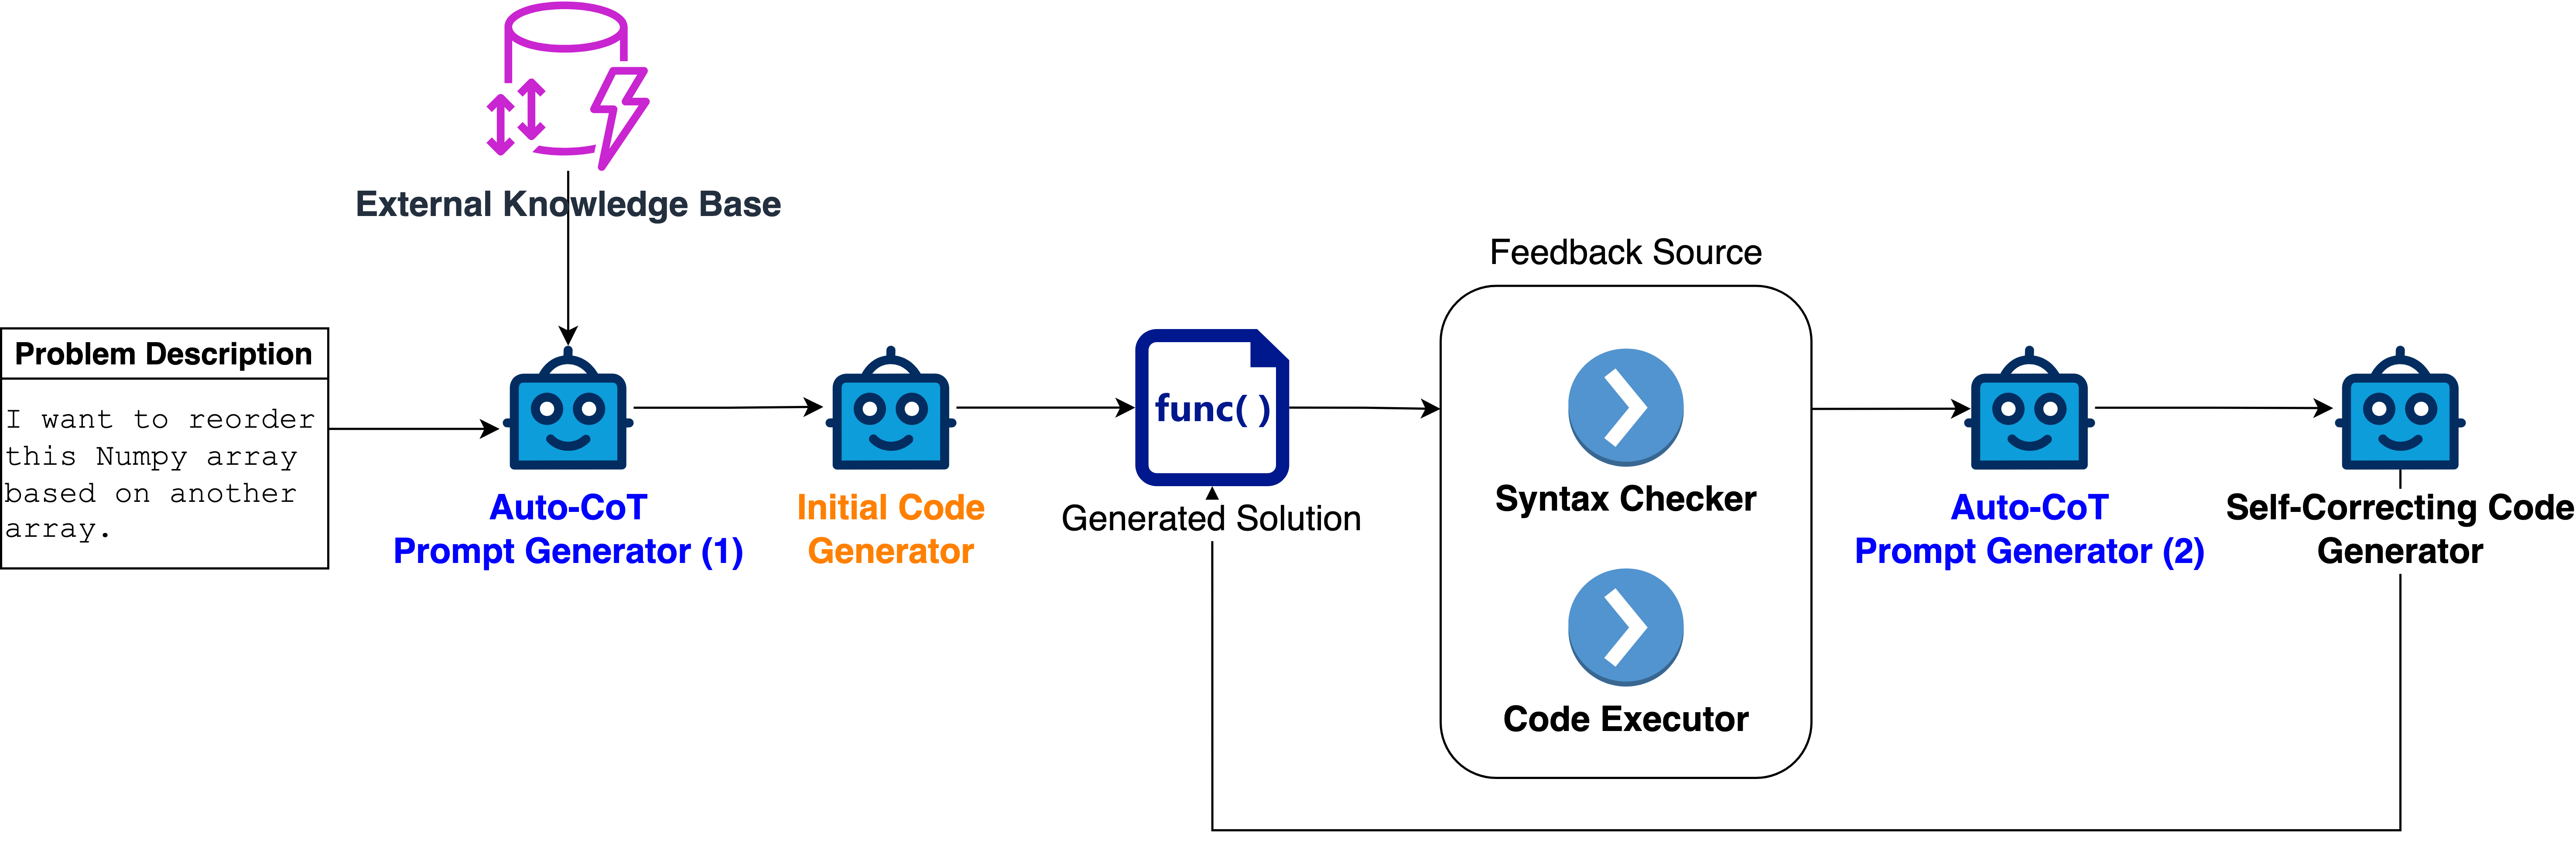
\includegraphics[width=0.8\textwidth]{img/cot_selfevolve_architecture}
        \captionsetup{font=small,labelformat=empty}
        \caption{Architecture of the CoT-SelfEvolve model (this study).}
    \end{figure}
\end{frame}

\section{Related Works}

\begin{frame}{Problem Formulation}
    \begin{block}{Problem}
        Given a set of problems (software bugs) be denoted as \( P = \{P_1, P_2, \ldots, P_N\} \), where each problem \( P_i \) is associated with a description \( D_i \) detailing the observed errors.\\

        Additionally, for each problem \( P_i \), there exist multiple unit tests \( U_{i,j} \) representing different test cases to validate the correctness of the fixed code. The model has access to these unit tests to guide the correction process.\\

        The goal is to maximize the `pass@k' metric, which is defined as the percentage of problems in the set for which the $k$ initial attempts at correction passes all associated unit tests successfully.
    \end{block}
\end{frame}

\begin{frame}{Taxonomy of Related Works}
    \begin{figure}
        \centering
        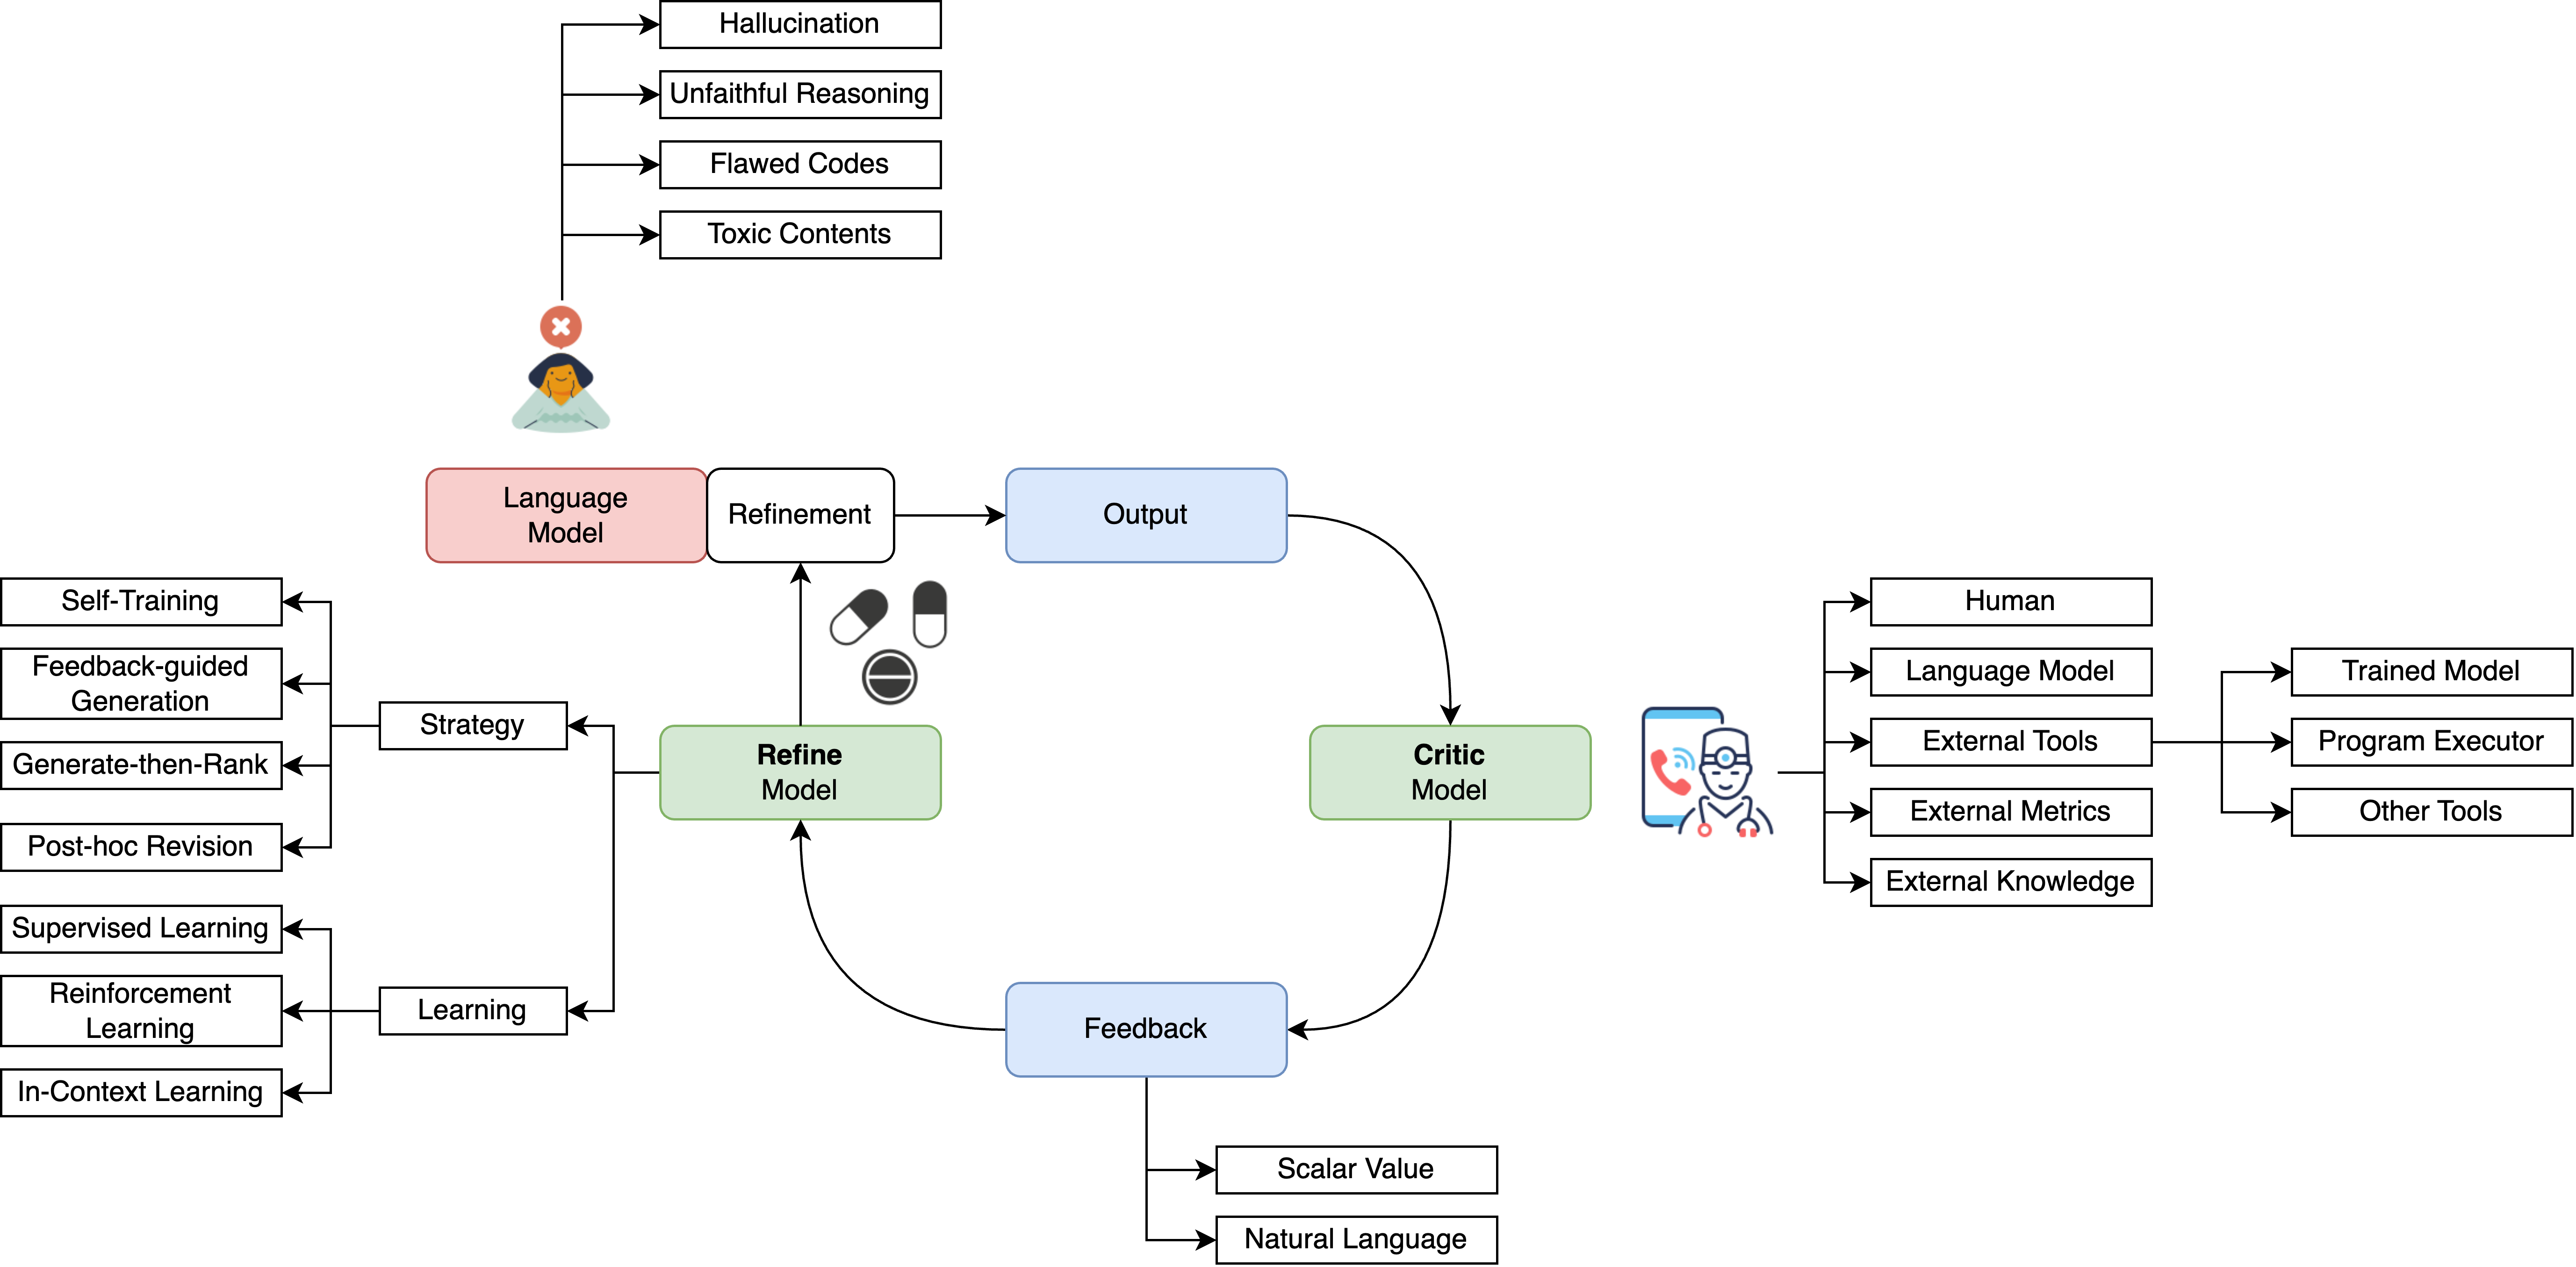
\includegraphics[scale=0.045]{img/taxonomy}
        \caption{Taxonomy of related works.}\label{fig:taxonomy}
    \end{figure}
    In Figure~\ref{fig:taxonomy}, a conceptual framework with three actors depicts related works: a \textbf{Language Model} generates initial output, a \textbf{Critic Model} analyzes and offers feedback, and a \textbf{Refine Model} adjusts either the output or the language model.
\end{frame}

\begin{frame}{Language Model}
    \begin{columns}[T]
        \begin{column}{0.70\textwidth}
            The works aimed at developing self-correcting LLMs can be classified according to the issues they tackle:
            \begin{enumerate}
                \item Hallucination: plausible-sounding but false information~\cite{gao2023rarr, zhang2023language}.

                \item Unfaithful Reasoning: derived conclusion does not follow the previously generated reasoning chain~\cite{he2022rethinking, pan2023logiclm}.

                \item Toxic Contents: content that is toxic, biased, or harmful due to biases present in the training datas~\cite{lu2022quark, gou2023critic}.

                \item Flawed Codes: flawed or incorrect code generation~\cite{chen2023teaching, olausson2023selfrepair}.
            \end{enumerate}
        \end{column}
        \begin{column}{0.30\textwidth}
            \begin{figure}[!htb]
                \centering
                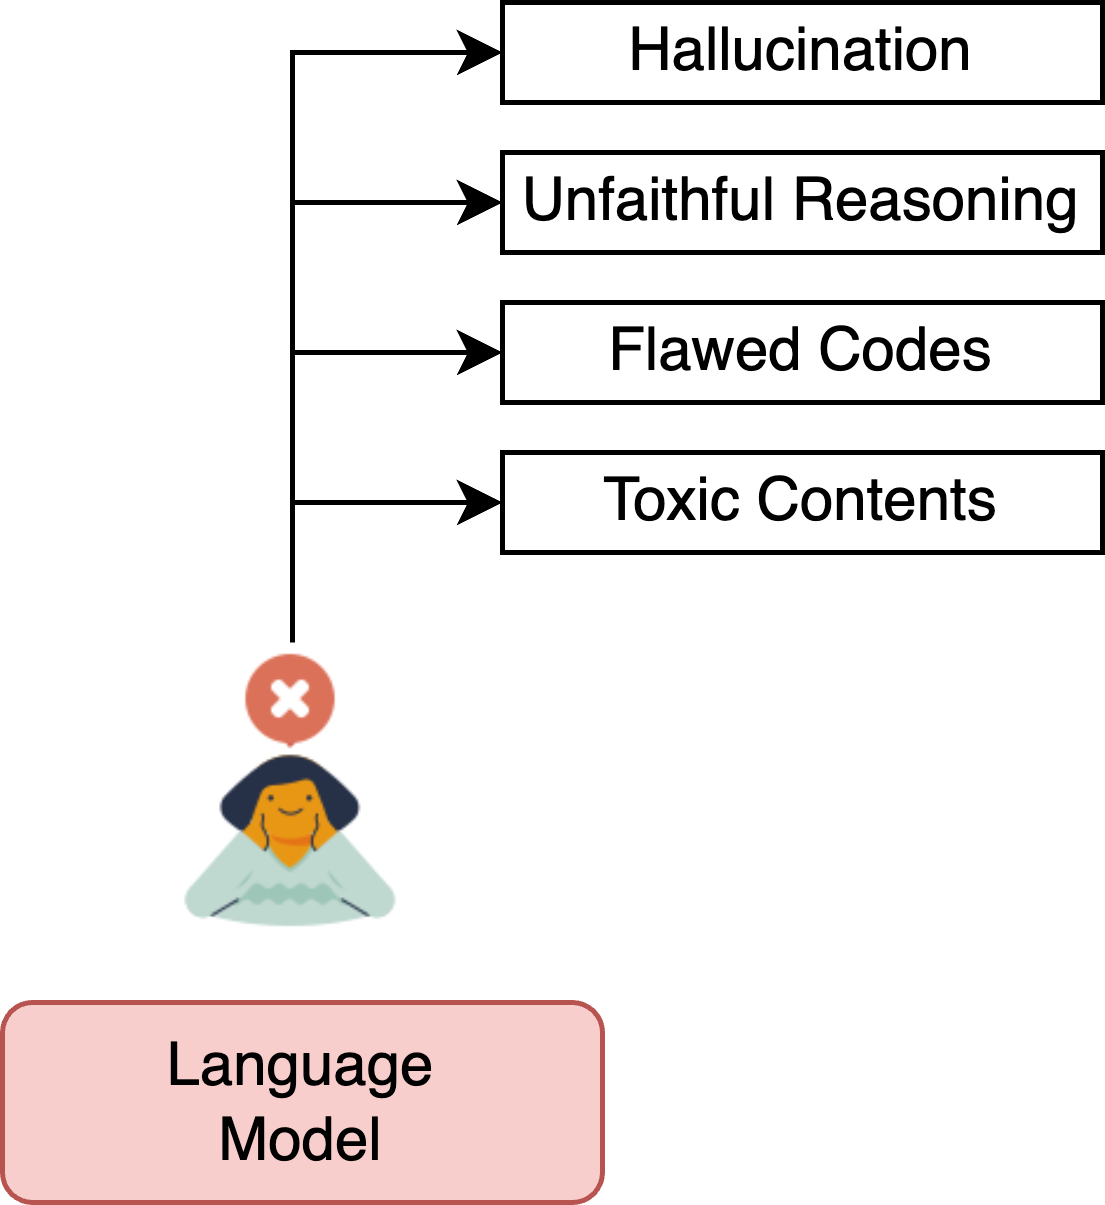
\includegraphics[scale=0.08]{img/language_model}
                \captionsetup{font=small}
                \caption{Problems of LLMs.}
            \end{figure}
        \end{column}
    \end{columns}
\end{frame}

\begin{frame}{Critic Model}
    \begin{columns}[T]
        \begin{column}{0.55\textwidth}
            Source of feedback:
            \begin{enumerate}
                \item Self-Feedback: the model itself generates feedback~\cite{weng2023large}.

                \item External Feedback: the model receives feedback from an external source (e.g., human, program executor and external knowledge)~\cite{gou2023critic}.
            \end{enumerate}

            Format of feedback:
            \begin{enumerate}
                \item Scalar Value: metrics based on pre-defined tests~\cite{weng2023large}.

                \item Natural Language: provides richer information than scalar value feedback~\cite{chen2023teaching}.
            \end{enumerate}
        \end{column}
        \begin{column}{0.45\textwidth}
            \begin{figure}[!htb]
                \centering
                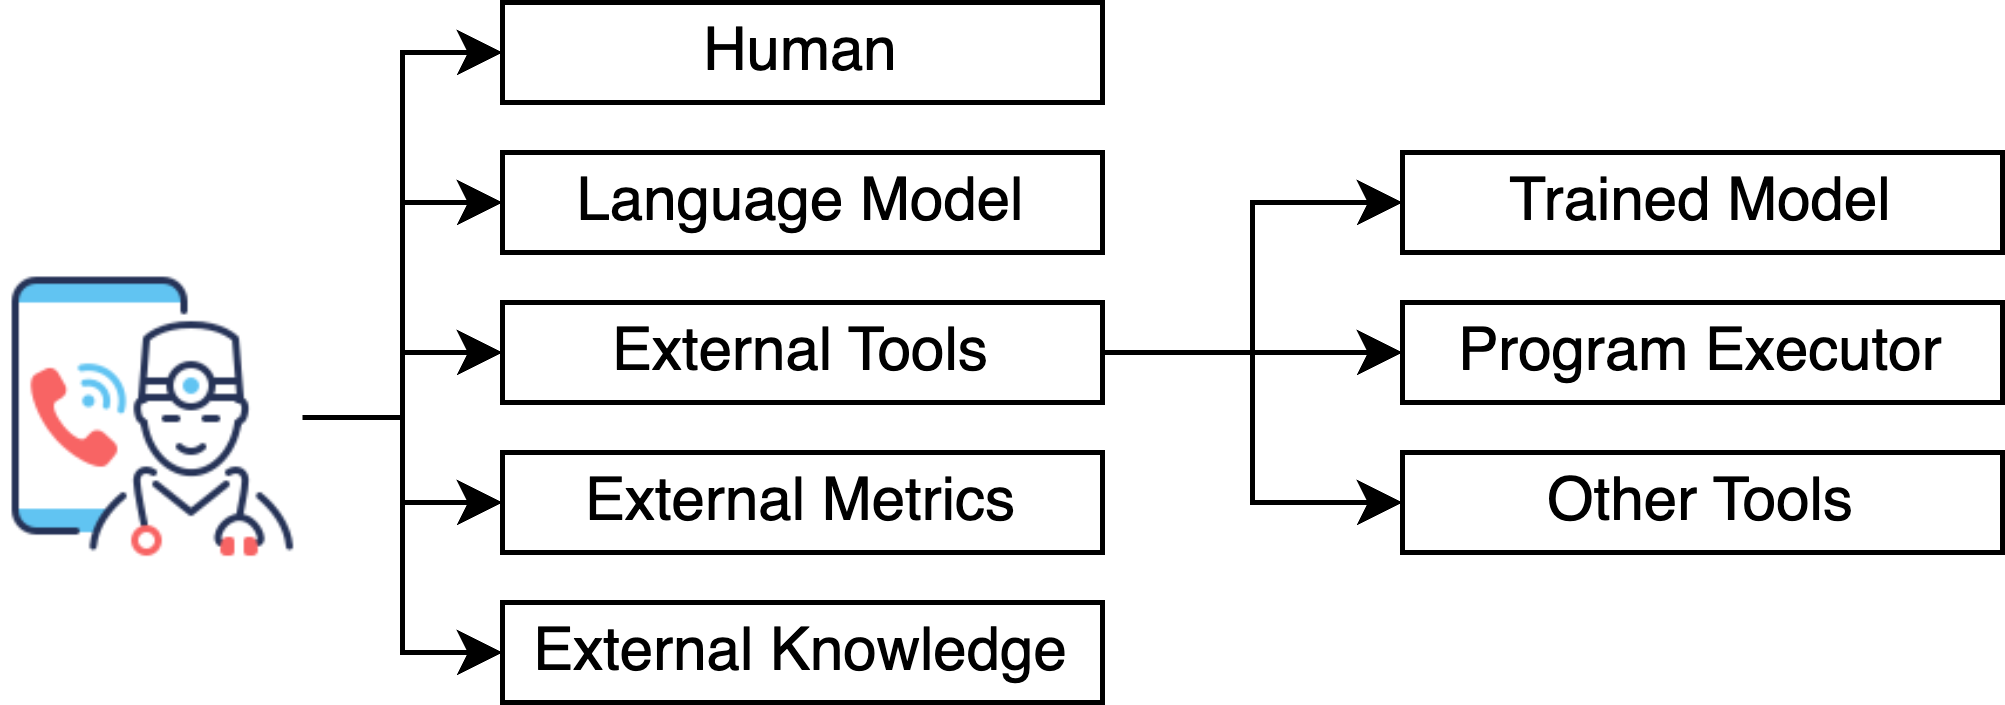
\includegraphics[scale=0.072]{img/critic_model}
                \captionsetup{font=small}
                \caption{Critic Model.}
            \end{figure}
        \end{column}
    \end{columns}
\end{frame}

\begin{frame}{Refine Model}
    The Refine Model is the most active area of research in the field. Existing works can be classified based on the following key questions:
    \begin{enumerate}
        \item Need to update the LLMs? \textbf{Yes}: Self-Training~\cite{huang2022large}, Supervised Learning~\cite{bai2022training}, Reinforcement Learning~\cite{dubois2024alpacafarm}, In-Context Learning~\cite{dong2022survey}.

        \item When to refine: generation-time or post-hoc?
              \begin{itemize}
                  \item Generation-time: Generate-then-Rank~\cite{cobbe2021training}, Feedback-Guided Generation~\cite{yao2023tree}.
                  \item Post-hoc: Models/Tools as Feedback~\cite{zhang2023selfedit}, Multi-Agent Debate~\cite{du2023improving}.
              \end{itemize}
    \end{enumerate}
\end{frame}

\section{Methodology}

\begin{frame}{Chain-of-Thought Prompting}
    \textit{Chain-of-Thought} (CoT) prompting~\cite{wei2023chainofthought}, which uses a series of intermediate reasoning steps, significantly improves the ability of LLMs to perform complex reasoning.\\
    \begin{figure}[!htb]
        \centering
        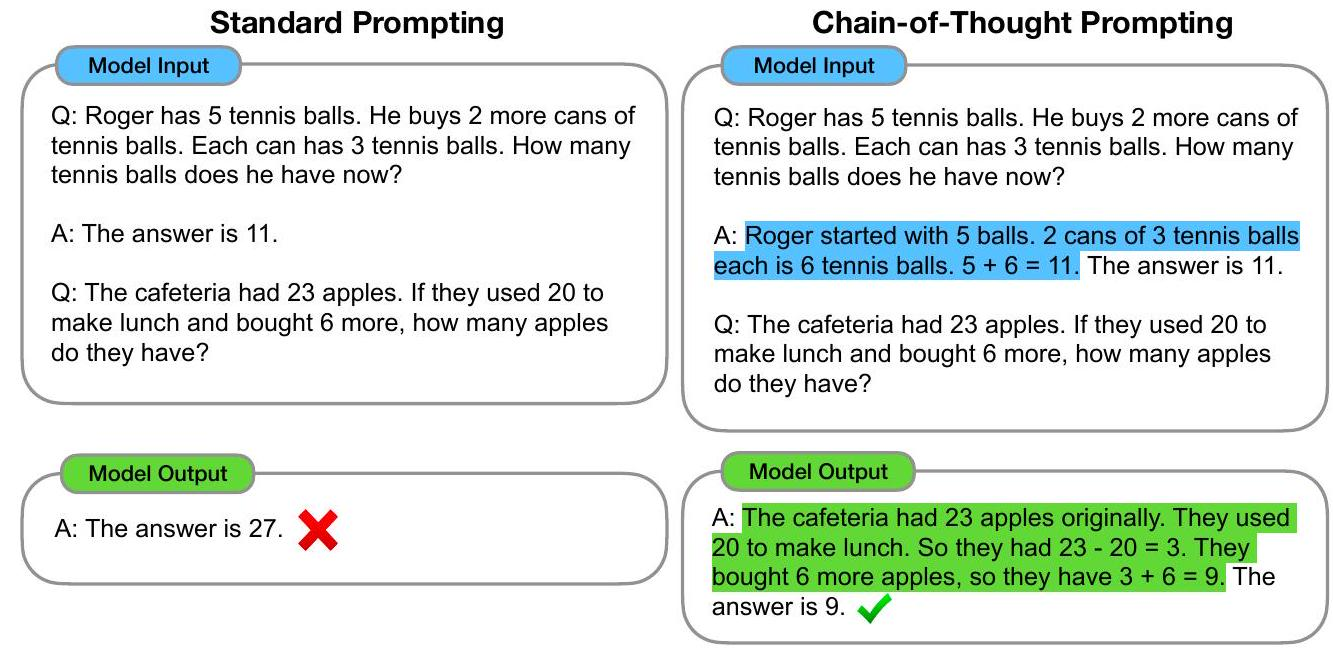
\includegraphics[width=0.75\textwidth]{img/cot_prompting}
        \captionsetup{font=small,labelformat=empty}
        \caption{Chain-of-Thought reasoning processes are highlighted.}
    \end{figure}
\end{frame}

\begin{frame}{CoT Techniques}
    \begin{figure}[!htb]
        \centering
        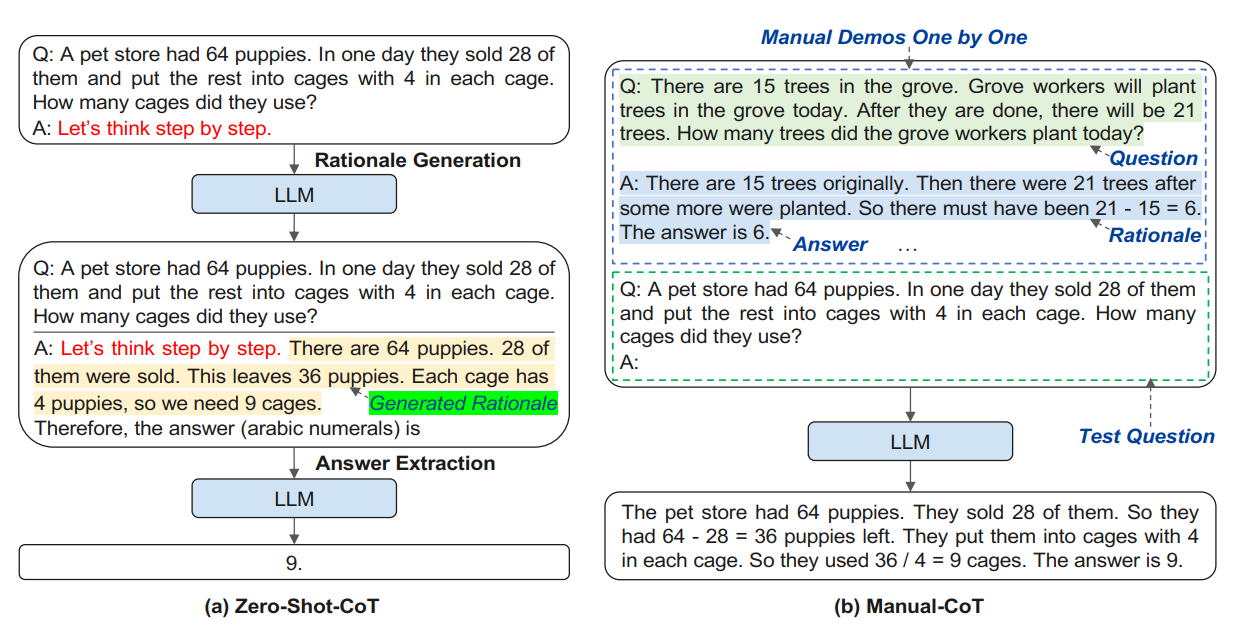
\includegraphics[width=\textwidth]{img/cot_types}
        \captionsetup{font=small,labelformat=empty}
        \caption{Zero-shot-CoT vs. Manual-CoT.}
    \end{figure}
\end{frame}

\begin{frame}{CoT Techniques}
    An automatic CoT prompting method (Auto-CoT~\cite{zhang2022automatic}), generates diverse samples and reasoning chains. In ten GPT-3 benchmark reasoning tasks, it consistently meets or surpasses manual CoT performance.
    \begin{figure}[!htb]
        \centering
        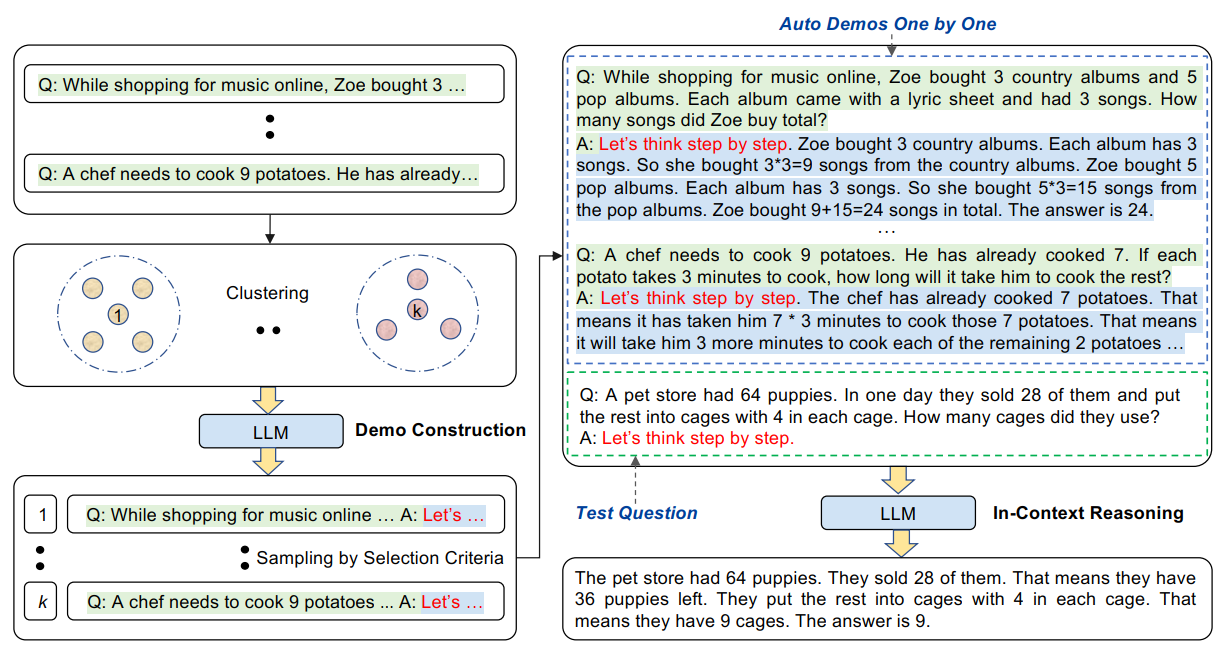
\includegraphics[width=0.85\textwidth]{img/auto_cot}
        \captionsetup{font=small,labelformat=empty}
        \caption{Auto-CoT.}
    \end{figure}
\end{frame}

\begin{frame}{CoT-SelfEvolve Architecture}
    \begin{figure}[!htb]
        \centering
        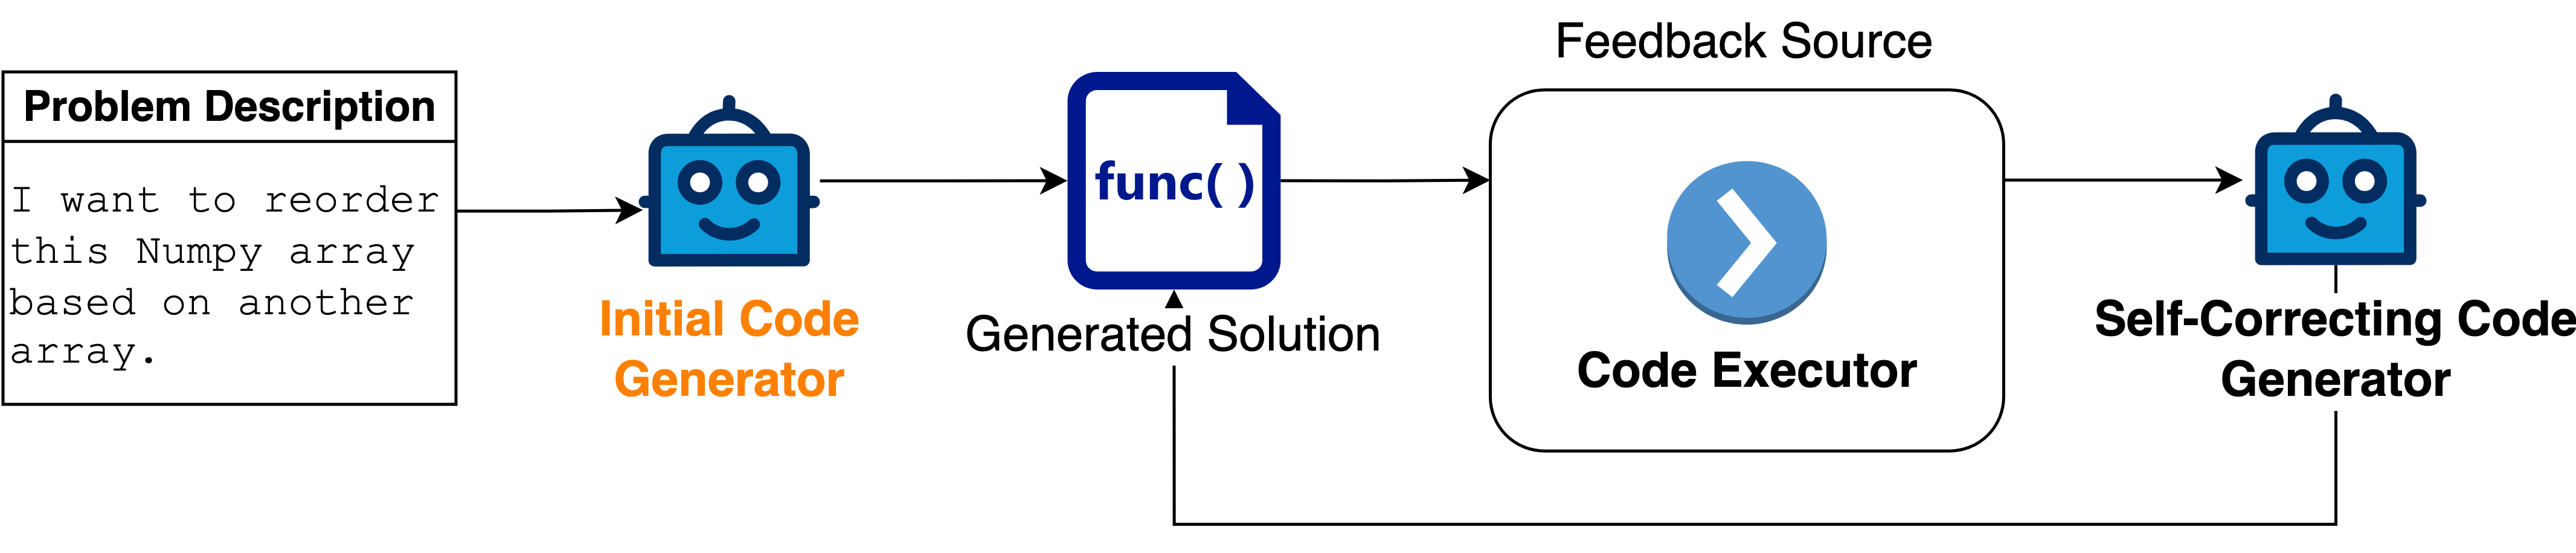
\includegraphics[width=0.70\textwidth]{img/selfevolve_architecture}
        \captionsetup{font=small,labelformat=empty}
        \caption{Architecture of the SelfEvolve~\cite{jiang2023selfevolve} model.}
    \end{figure}
    \begin{figure}[!htb]
        \centering
        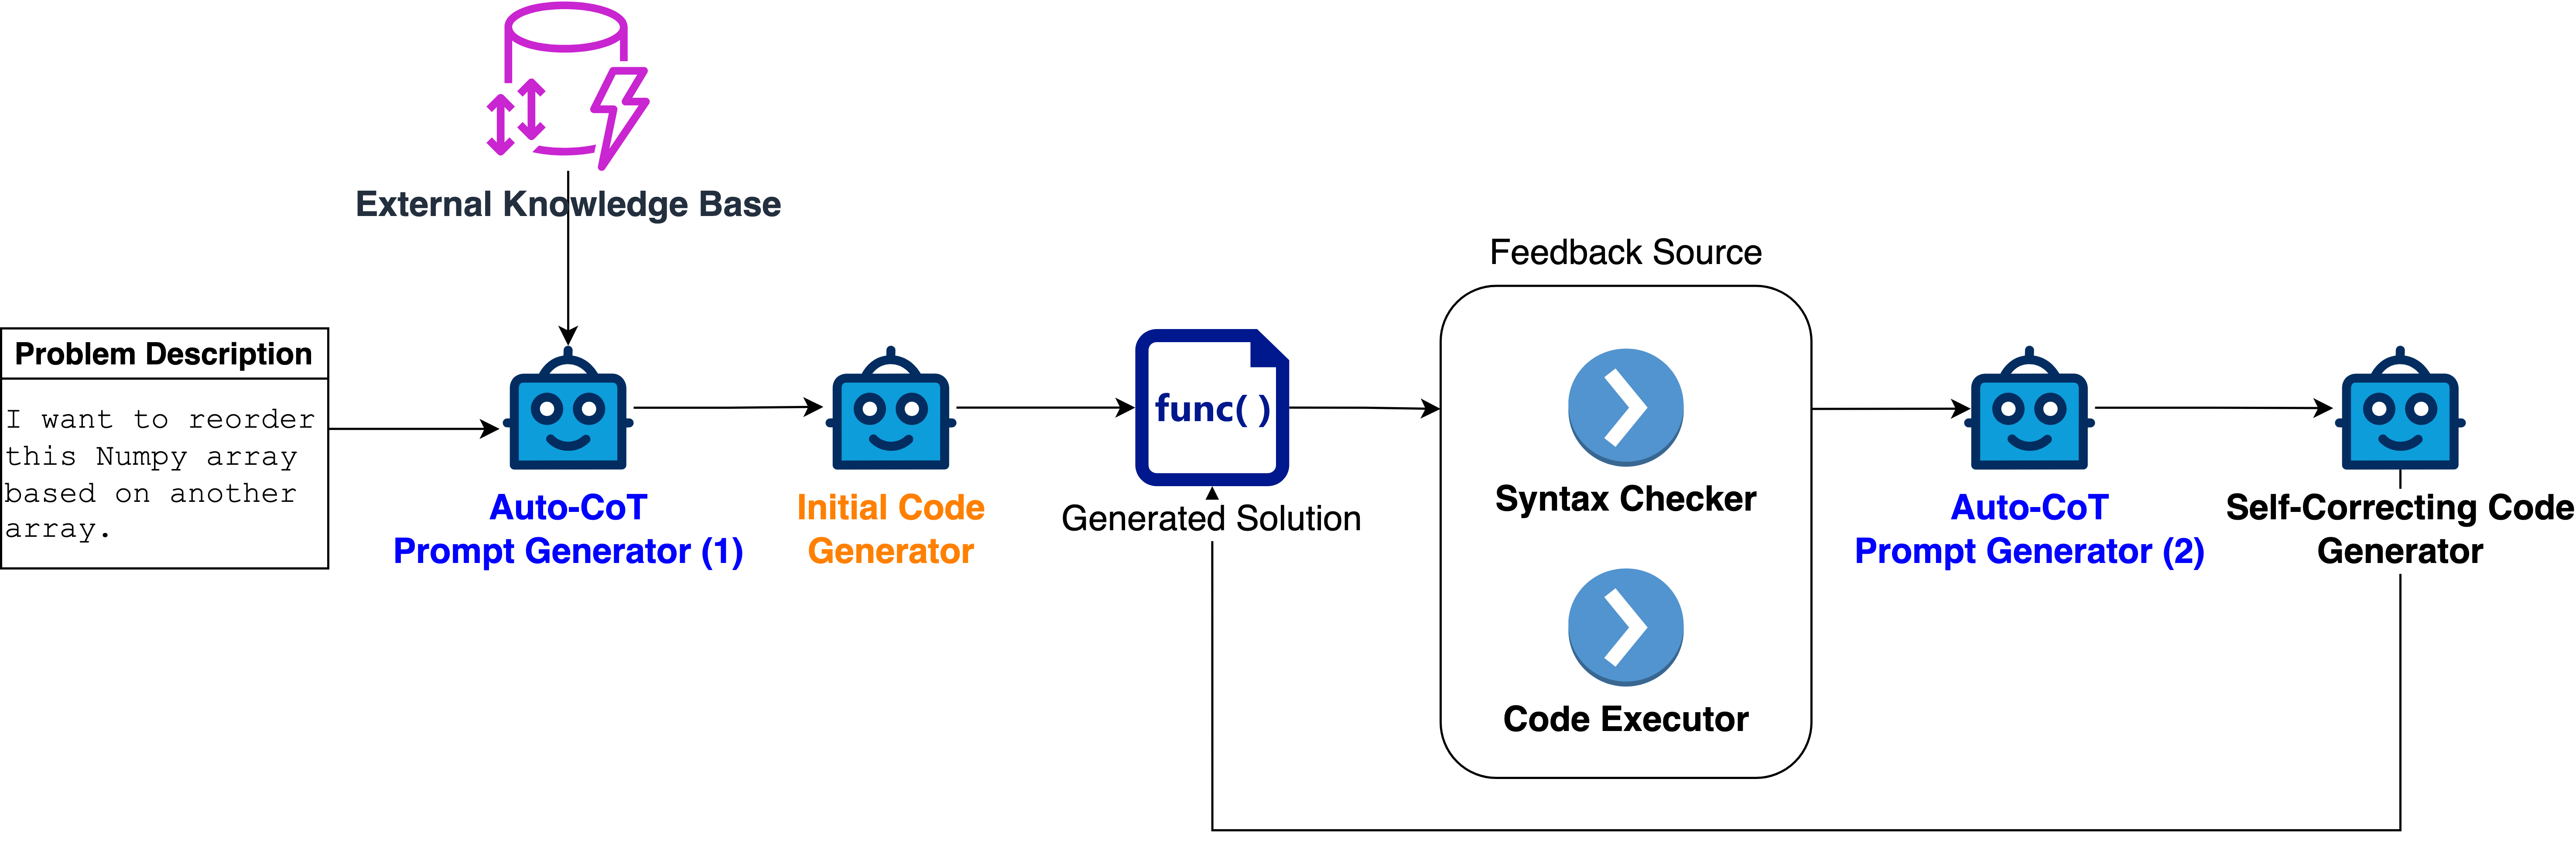
\includegraphics[width=0.90\textwidth]{img/cot_selfevolve_architecture}
        \captionsetup{font=small,labelformat=empty}
        \caption{Architecture of the CoT-SelfEvolve model (this study).}
    \end{figure}
\end{frame}

\begin{frame}{Auto-CoT Prompt Generation (1)}
    The initial Auto-CoT prompt generator integrates problem descriptions with relevant StackOverflow discussions. This in-context material aids a LLM in reasoning and hint generation for problem-solving. These hints then serve as CoT prompts for another LLM (Code Generator).
    \begin{figure}[!htb]
        \centering
        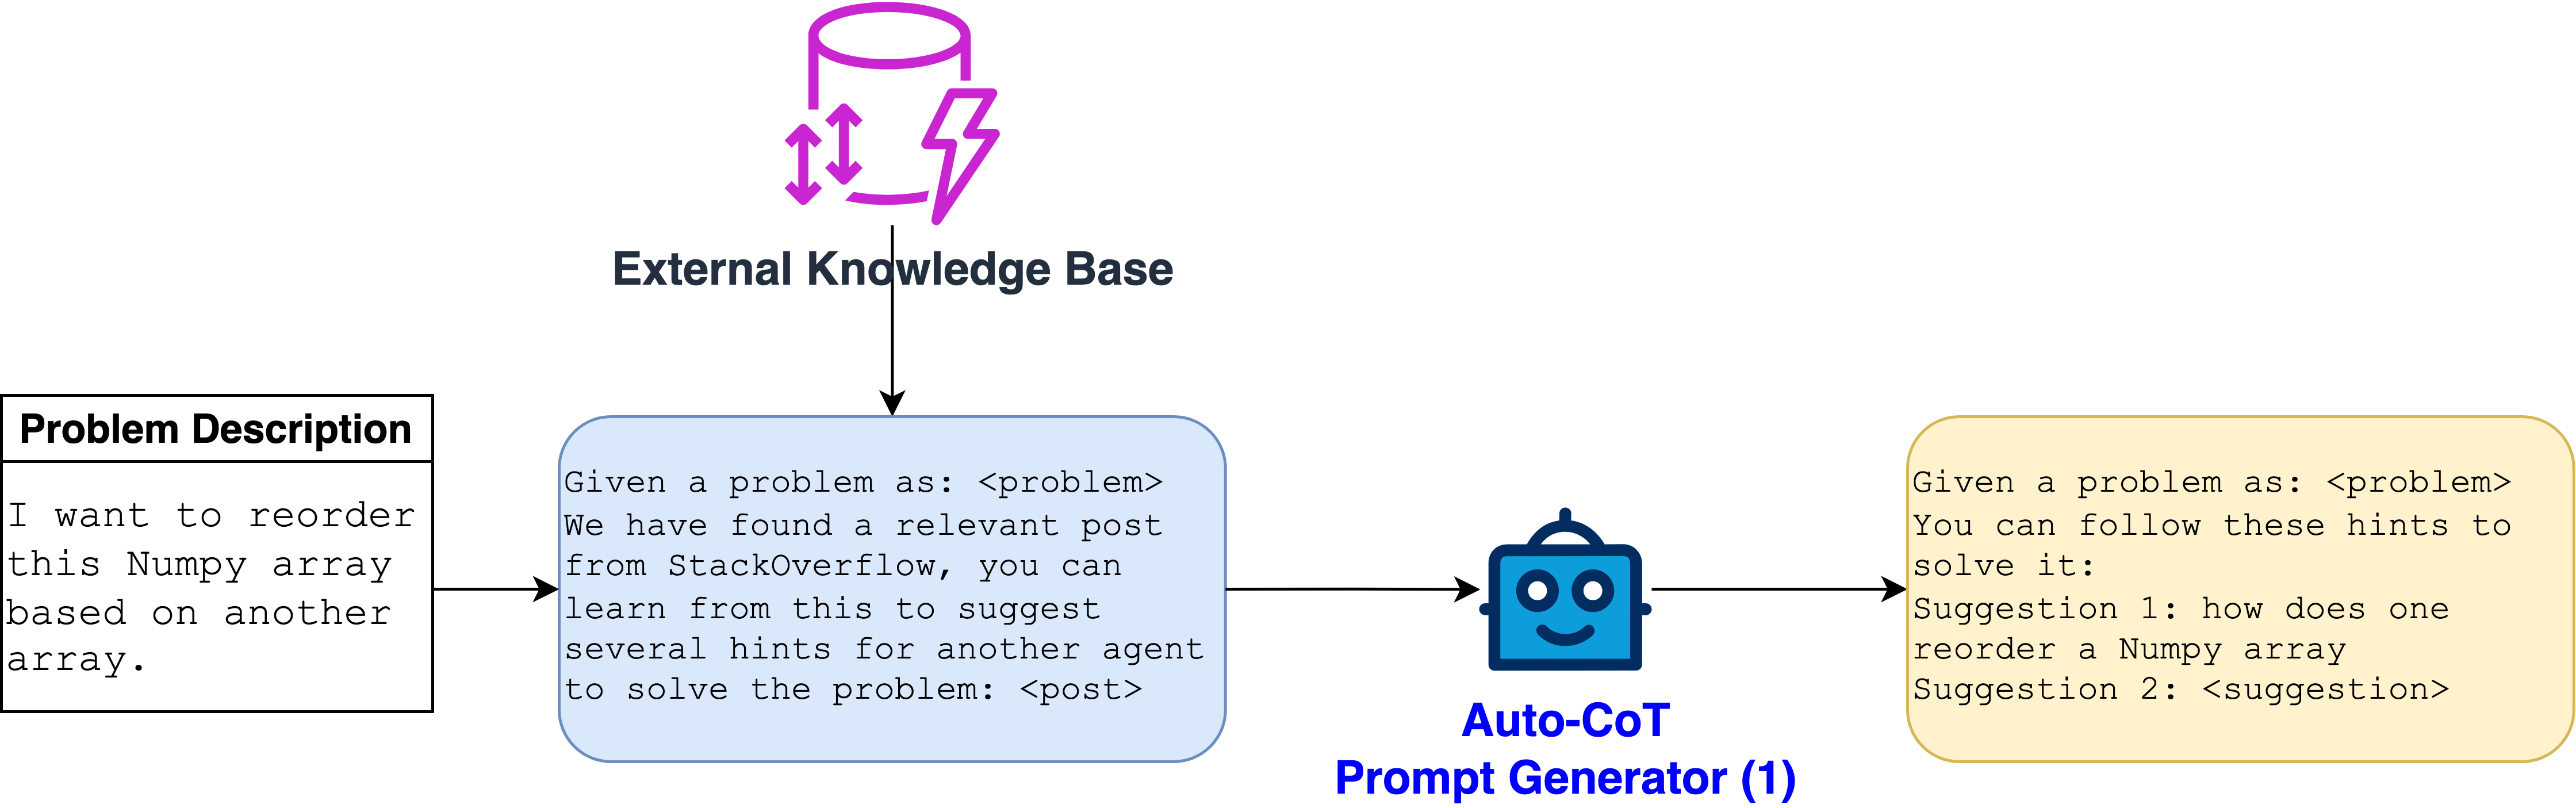
\includegraphics[width=\textwidth]{img/cot_generator_1}
        \captionsetup{font=small,labelformat=empty}
        \caption{Auto-CoT Prompt Generation (1).}
    \end{figure}
\end{frame}

\begin{frame}{Auto-CoT Prompt Generation (2)}
    The second Auto-CoT prompt generator combines problem descriptions with feedback from syntax checkers or code executors. It aims to generate self-reflective questions for a LLM to consider during problem-solving.
    \begin{figure}[!htb]
        \centering
        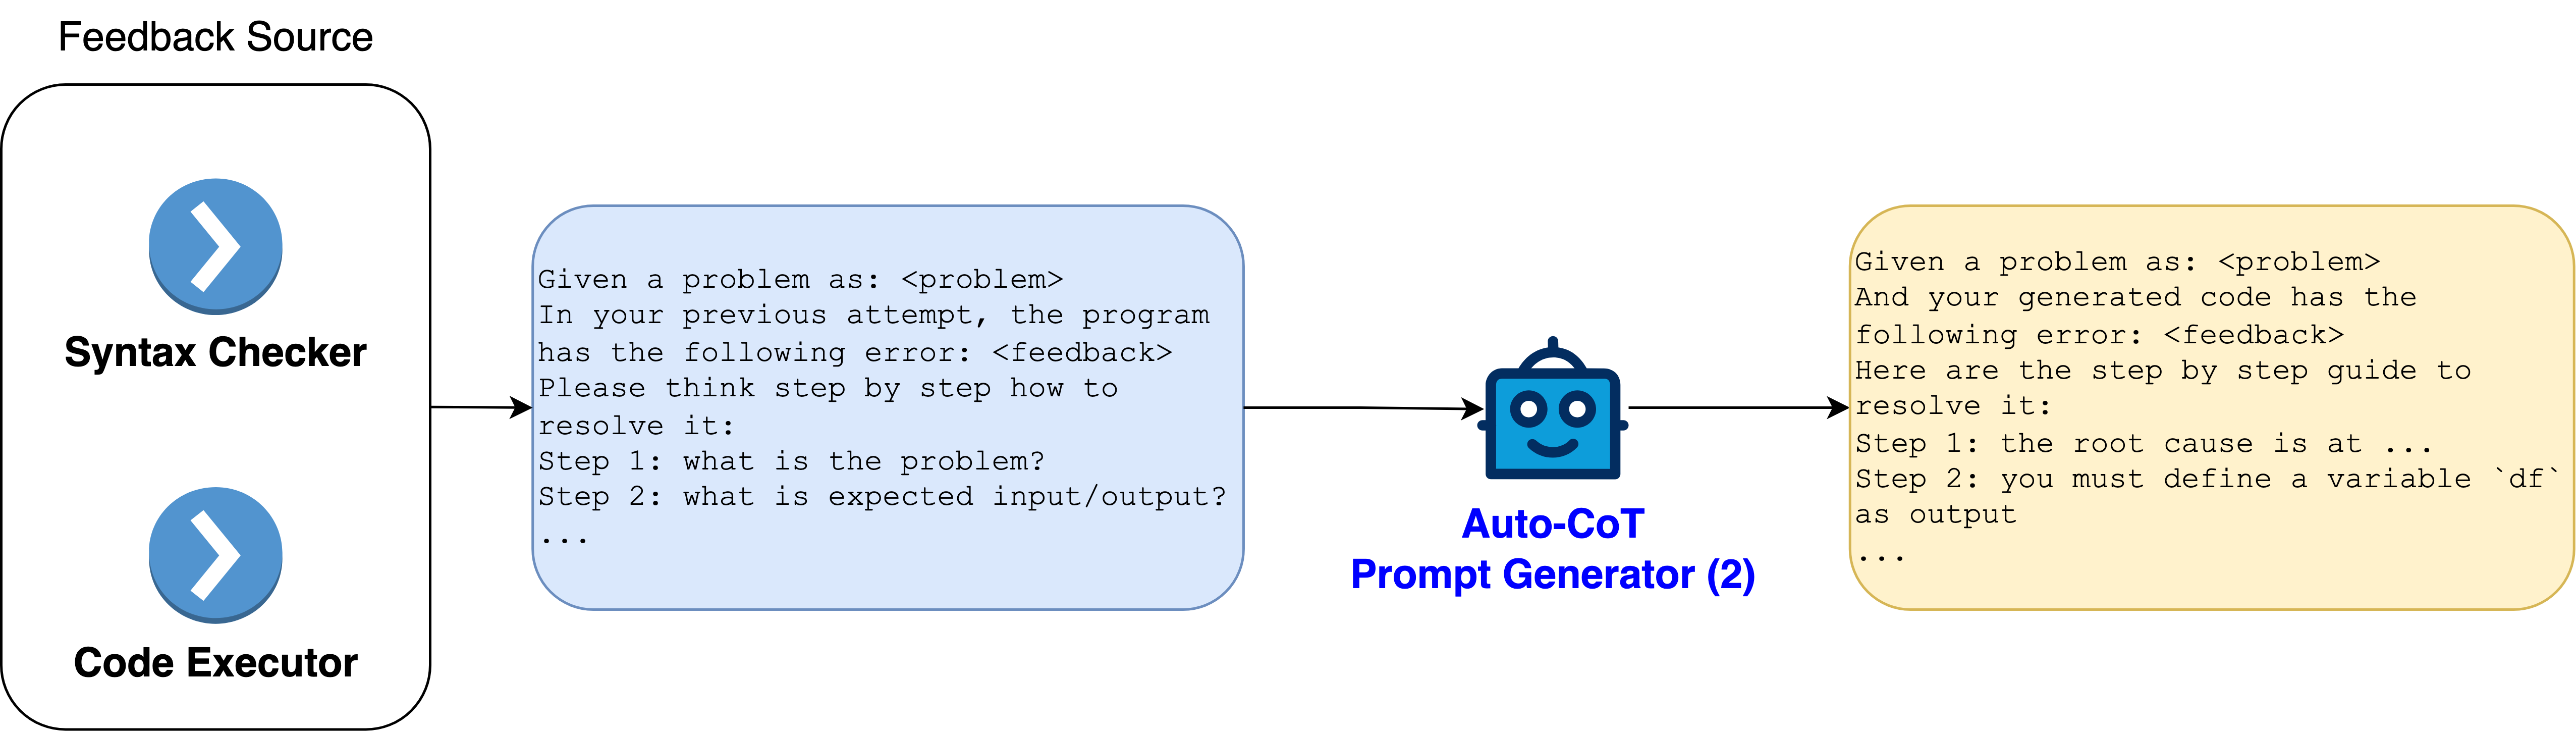
\includegraphics[width=\textwidth]{img/cot_generator_2}
        \captionsetup{font=small,labelformat=empty}
        \caption{Auto-CoT Prompt Generation (2).}
    \end{figure}
\end{frame}

\begin{frame}{External Knowledge Base}
    \begin{columns}[T] % align columns
        \begin{column}{.4\textwidth}
            \begin{figure}[!htb]
                \centering
                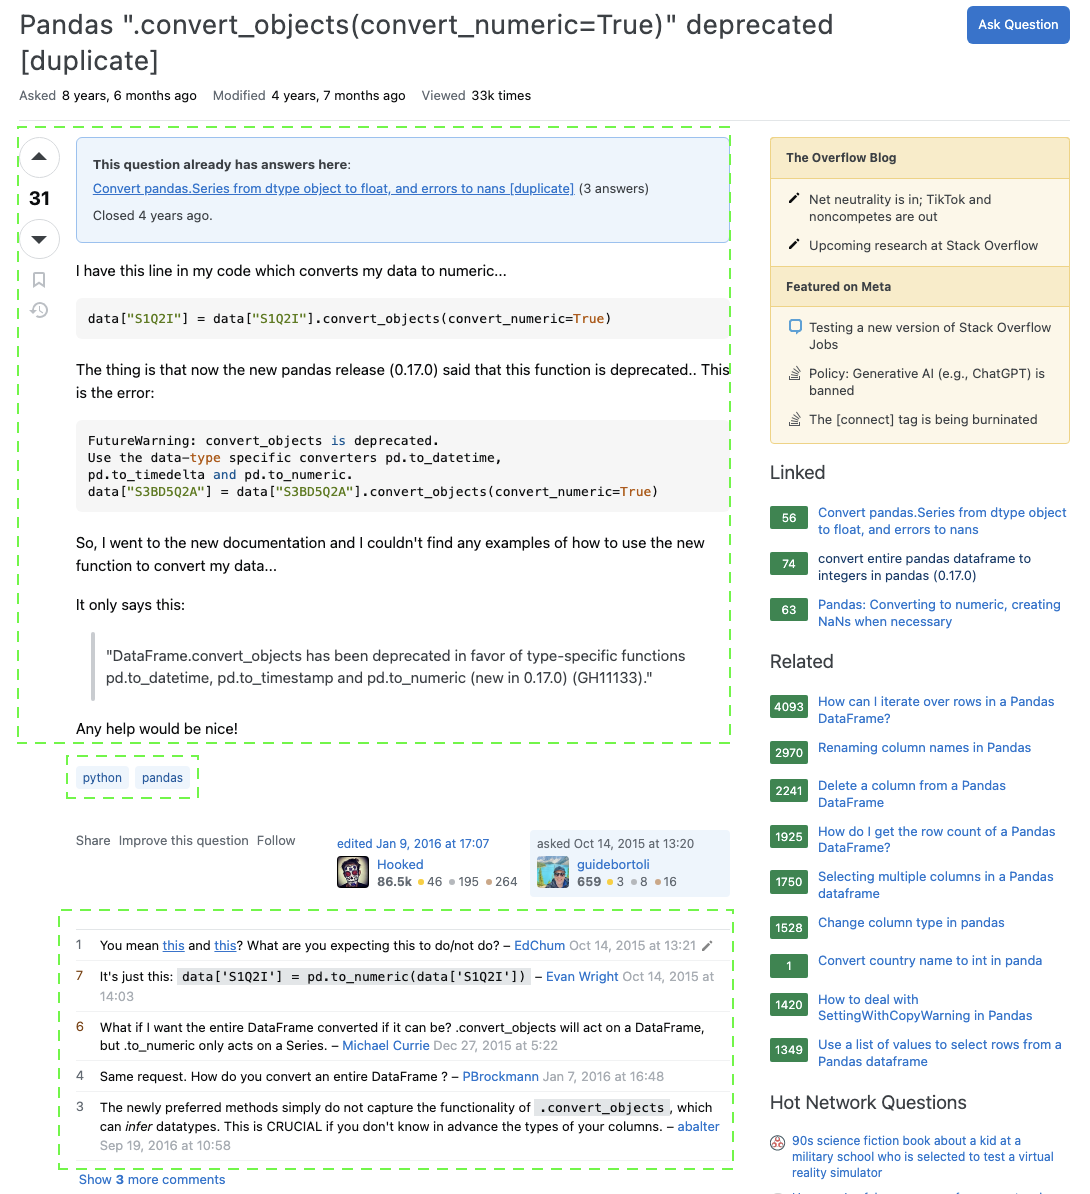
\includegraphics[width=\textwidth]{img/stackoverflow.png}
                \captionsetup{font=small,labelformat=empty}
                \caption{Example of StackOverflow discussions.}
            \end{figure}
        \end{column}%
        \begin{column}{.6\textwidth}
            \begin{itemize}
                \item An external knowledge base, narrowed to seven Python libraries, is constructed from 500,000 StackOverflow discussions.
                \item Each document amalgamates a problem description with its comments.
                \item OpenAI's text-embedding-ada-02 model generates the embeddings.
                \item Using the HNSW algorithm on top of these embeddings to retrieve relevant documents for a specific problem.
            \end{itemize}
        \end{column}%
    \end{columns}
\end{frame}

\section{Benchmark Dataset}

\begin{frame}{DS-1000}
    DS-1000~\cite{pmlr-v202-lai23b}: 1000 Python data science coding problems, each with:
    \begin{block}{Problem Description}
        \small
        Problem:
        How do I get the dimensions of an array? For instance, this is (2, 2):\\
        a = np.array([[1,2],[3,4]])
    \end{block}

    \begin{columns}[T]
        \begin{column}{0.50\textwidth}
            \begin{block}{Code Context}
                \small
                <code>\\
                import numpy as np\\
                a = np.array([[1,2],[3,4]])\\
                </code>\\
                result = $\ldots$ \# put solution in this variable\\
                BEGIN SOLUTION\\
                <code>
            \end{block}
        \end{column}
        \begin{column}{0.45\textwidth}
            \begin{block}{Unit Test}
                \small
                def test(result, ans):\\
                \ \ \ \ assert\_array\_equal(result, ans)\\
                \ \ \ \ return 1
            \end{block}
        \end{column}
    \end{columns}
\end{frame}

\begin{frame}{Evalution Metric}
    \begin{columns}[T] % align columns
        \begin{column}{.5\textwidth}
            The SelfEvolve model employs the `pass@1' metric, which is the ratio of correctly solved problems to total problems, \textit{with a few refinement steps}.
        \end{column}%
        \begin{column}{.5\textwidth}
            In this study, the CoT-SelfEvolve model is allowed to try maximum 5 attepmts to solve a problem, thus, the metric is `pass@5'.
        \end{column}%
    \end{columns}
\end{frame}

\section{Experiments and Results}

\begin{frame}{Experiments}
    Four types of experiments were conducted, each involving a single pass through 1000 problems due to cost constraints.

    \begin{enumerate}
        \item \textbf{Full System:} The CoT-SelfEvolve model was evaluated alongside six different Language Learning Models (LLMs), including GPT-3.5-turbo, GPT-4, Claude 2.1, Claude 3, Mistral Large, and Mistral 8x7B.

        \item \textbf{Auto-CoT Generators:} The functionality of Auto-CoT generators was toggled on and off to examine their impact on the performance of CoT-SelfEvolve.

        \item \textbf{Large LLM as Teacher:} A large LLM, such as GPT-4, was used for CoT prompt generation, while GPT-3.5-turbo was used for code generation.

        \item \textbf{Auto-CoT with Code LLM:} The initial Auto-CoT prompt generator was evaluated using the specialized code LLM (Llama 3 70B).
    \end{enumerate}
\end{frame}

\begin{frame}{Result: Full System}
    The CoT-SelfEvolve model, employing GPT-4 as the base LLM, outperformed the original SelfEvolve model in handling Pytorch, Sklearn, and Matplotlib questions, demonstrating a clear superiority.

    \begin{table}[H]
        \caption*{$\text{Pass@5}$ results on the DS-1000 dataset. (\%)}
        \resizebox{\textwidth}{!}{%
            \begin{tabular}{|l|l|c|c|c|c|c|c|c|c|}
                \hline
                                                & LLM           & \multicolumn{1}{l|}{Scipy} & \multicolumn{1}{l|}{PyTorch} & \multicolumn{1}{l|}{Sklearn} & \multicolumn{1}{l|}{Matplotlib} & \multicolumn{1}{l|}{Pandas} & \multicolumn{1}{l|}{Numpy} & \multicolumn{1}{l|}{TensorFlow} & \multicolumn{1}{l|}{Overall} \\ \hline
                \multirow{2}{*}{SelfEvolve}     & GPT-3.5       & 52.83                      & 64.71                        & 73.04                        & 78.06                           &                             &                            &                                 & \multicolumn{1}{l|}{}        \\ \cline{2-10}
                                                & GPT-4         & \textbf{58.49}             & 70.59                        & 70.43                        & 84.52                           &                             &                            &                                 & \multicolumn{1}{l|}{}        \\ \hline
                \multirow{6}{*}{CoT-SelfEvolve} & GPT-3.5       & 32.08                      & 72.06                        & 66.09                        & 32.26                           & 29.55                       & 17.73                      & 46.67                           & 35.5                         \\ \cline{2-10}
                                                & GPT-4         & 53.77                      & \textbf{89.71}               & \textbf{97.39}               & \textbf{85.16}                  & \textbf{92.78}              & \textbf{76.36}             & \textbf{84.44}                  & \textbf{83.8}                \\ \cline{2-10}
                                                & Claude 2.1    & 47.17                      & 83.82                        & 85.22                        & 83.23                           & 65.64                       & 61.82                      & 57.78                           & 68.7                         \\ \cline{2-10}
                                                & Claude 3      & 44.34                      & 76.47                        & 73.91                        & 85.81                           & 43.64                       & 31.36                      & 53.33                           & 53.7                         \\ \cline{2-10}
                                                & Mistral Large & 45.28                      & 80.88                        & 78.26                        & 52.26                           & 68.04                       & 43.64                      & 53.33                           & 59.2                         \\ \cline{2-10}
                                                & Mistral 8x7B  & 30.19                      & 57.35                        & 56.52                        & 69.68                           & 38.49                       & 35.91                      & 44.44                           & 45.5                         \\ \hline
            \end{tabular}%
        }
    \end{table}
\end{frame}

\begin{frame}{Result: Auto-CoT Generators}
    The performance enhancement brought about by the Auto-CoT prompt generators is evident when compared to the non-CoT prompt version, with a relative gain of \textbf{16.39\%}. This finding highlights the significance of Auto-CoT prompt generators in augmenting the efficacy of the CoT-SelfEvolve model.

    \begin{table}[H]
        \caption*{$\text{Pass@5}$ results on the DS-1000 dataset w or w/o CoT prompts. (\%)}
        \resizebox{\textwidth}{!}{%
            \begin{tabular}{|c|c|c|c|c|c|c|c|c|c|}
                \hline
                Auto-CoT 1 & Auto-CoT 2 & Scipy & PyTorch & Sklearn & Matplotlib & Pandas & Numpy & TensorFlow & Overall \\ \hline
                off        & off        & 33.02 & 64.71   & 59.13   & 26.45      & 23.02  & 14.09 & 42.22      & 30.5    \\ \hline
                on         & off        & 28.3  & 75      & 63.48   & 29.68      & 29.21  & 17.27 & 51.11      & 34.6    \\ \hline
                on         & on         & 32.08 & 72.06   & 66.09   & 32.26      & 29.55  & 17.73 & 46.67      & 35.5    \\ \hline
                off        & on         & 23.58 & 66.18   & 53.91   & 29.68      & 30.24  & 18.18 & 42.22      & 32.4    \\ \hline
            \end{tabular}%
        }
    \end{table}
\end{frame}

\begin{frame}{Result: Large LLM as Teacher}
    The data clearly shows that leveraging a larger LLM to steer the code generation process can significantly enhance the model's performance, as evidenced by a relative gain of \textbf{11.26\%}.

    \begin{table}[H]
        \caption*{$\text{Pass@5}$ results on the DS-1000 dataset with different LLM stacks. (\%)}
        \centering
        \resizebox{\columnwidth}{!}{%
            \begin{tabular}{|c|c|c|c|c|c|c|c|c|c|}
                \hline
                Auto-CoT LLM & Code LLM & Scipy & PyTorch & Sklearn & Matplotlib & Pandas & Numpy & TensorFlow & Overall \\ \hline
                GPT-3.5 & GPT-3.5  & 32.08 & 72.06   & 66.09   & 32.26      & 29.55  & 17.73 & 46.67      & 35.5    \\ \hline
                GPT-4   & GPT-3.5  & 37.74 & 83.82   & 73.04   & 35.48      & 31.62  & 19.55 & 53.33      & 39.5    \\ \hline
            \end{tabular}%
        }
    \end{table}
\end{frame}

\begin{frame}{Result: Auto-CoT with Code LLM}
    \begin{figure}[H]
        \centering
        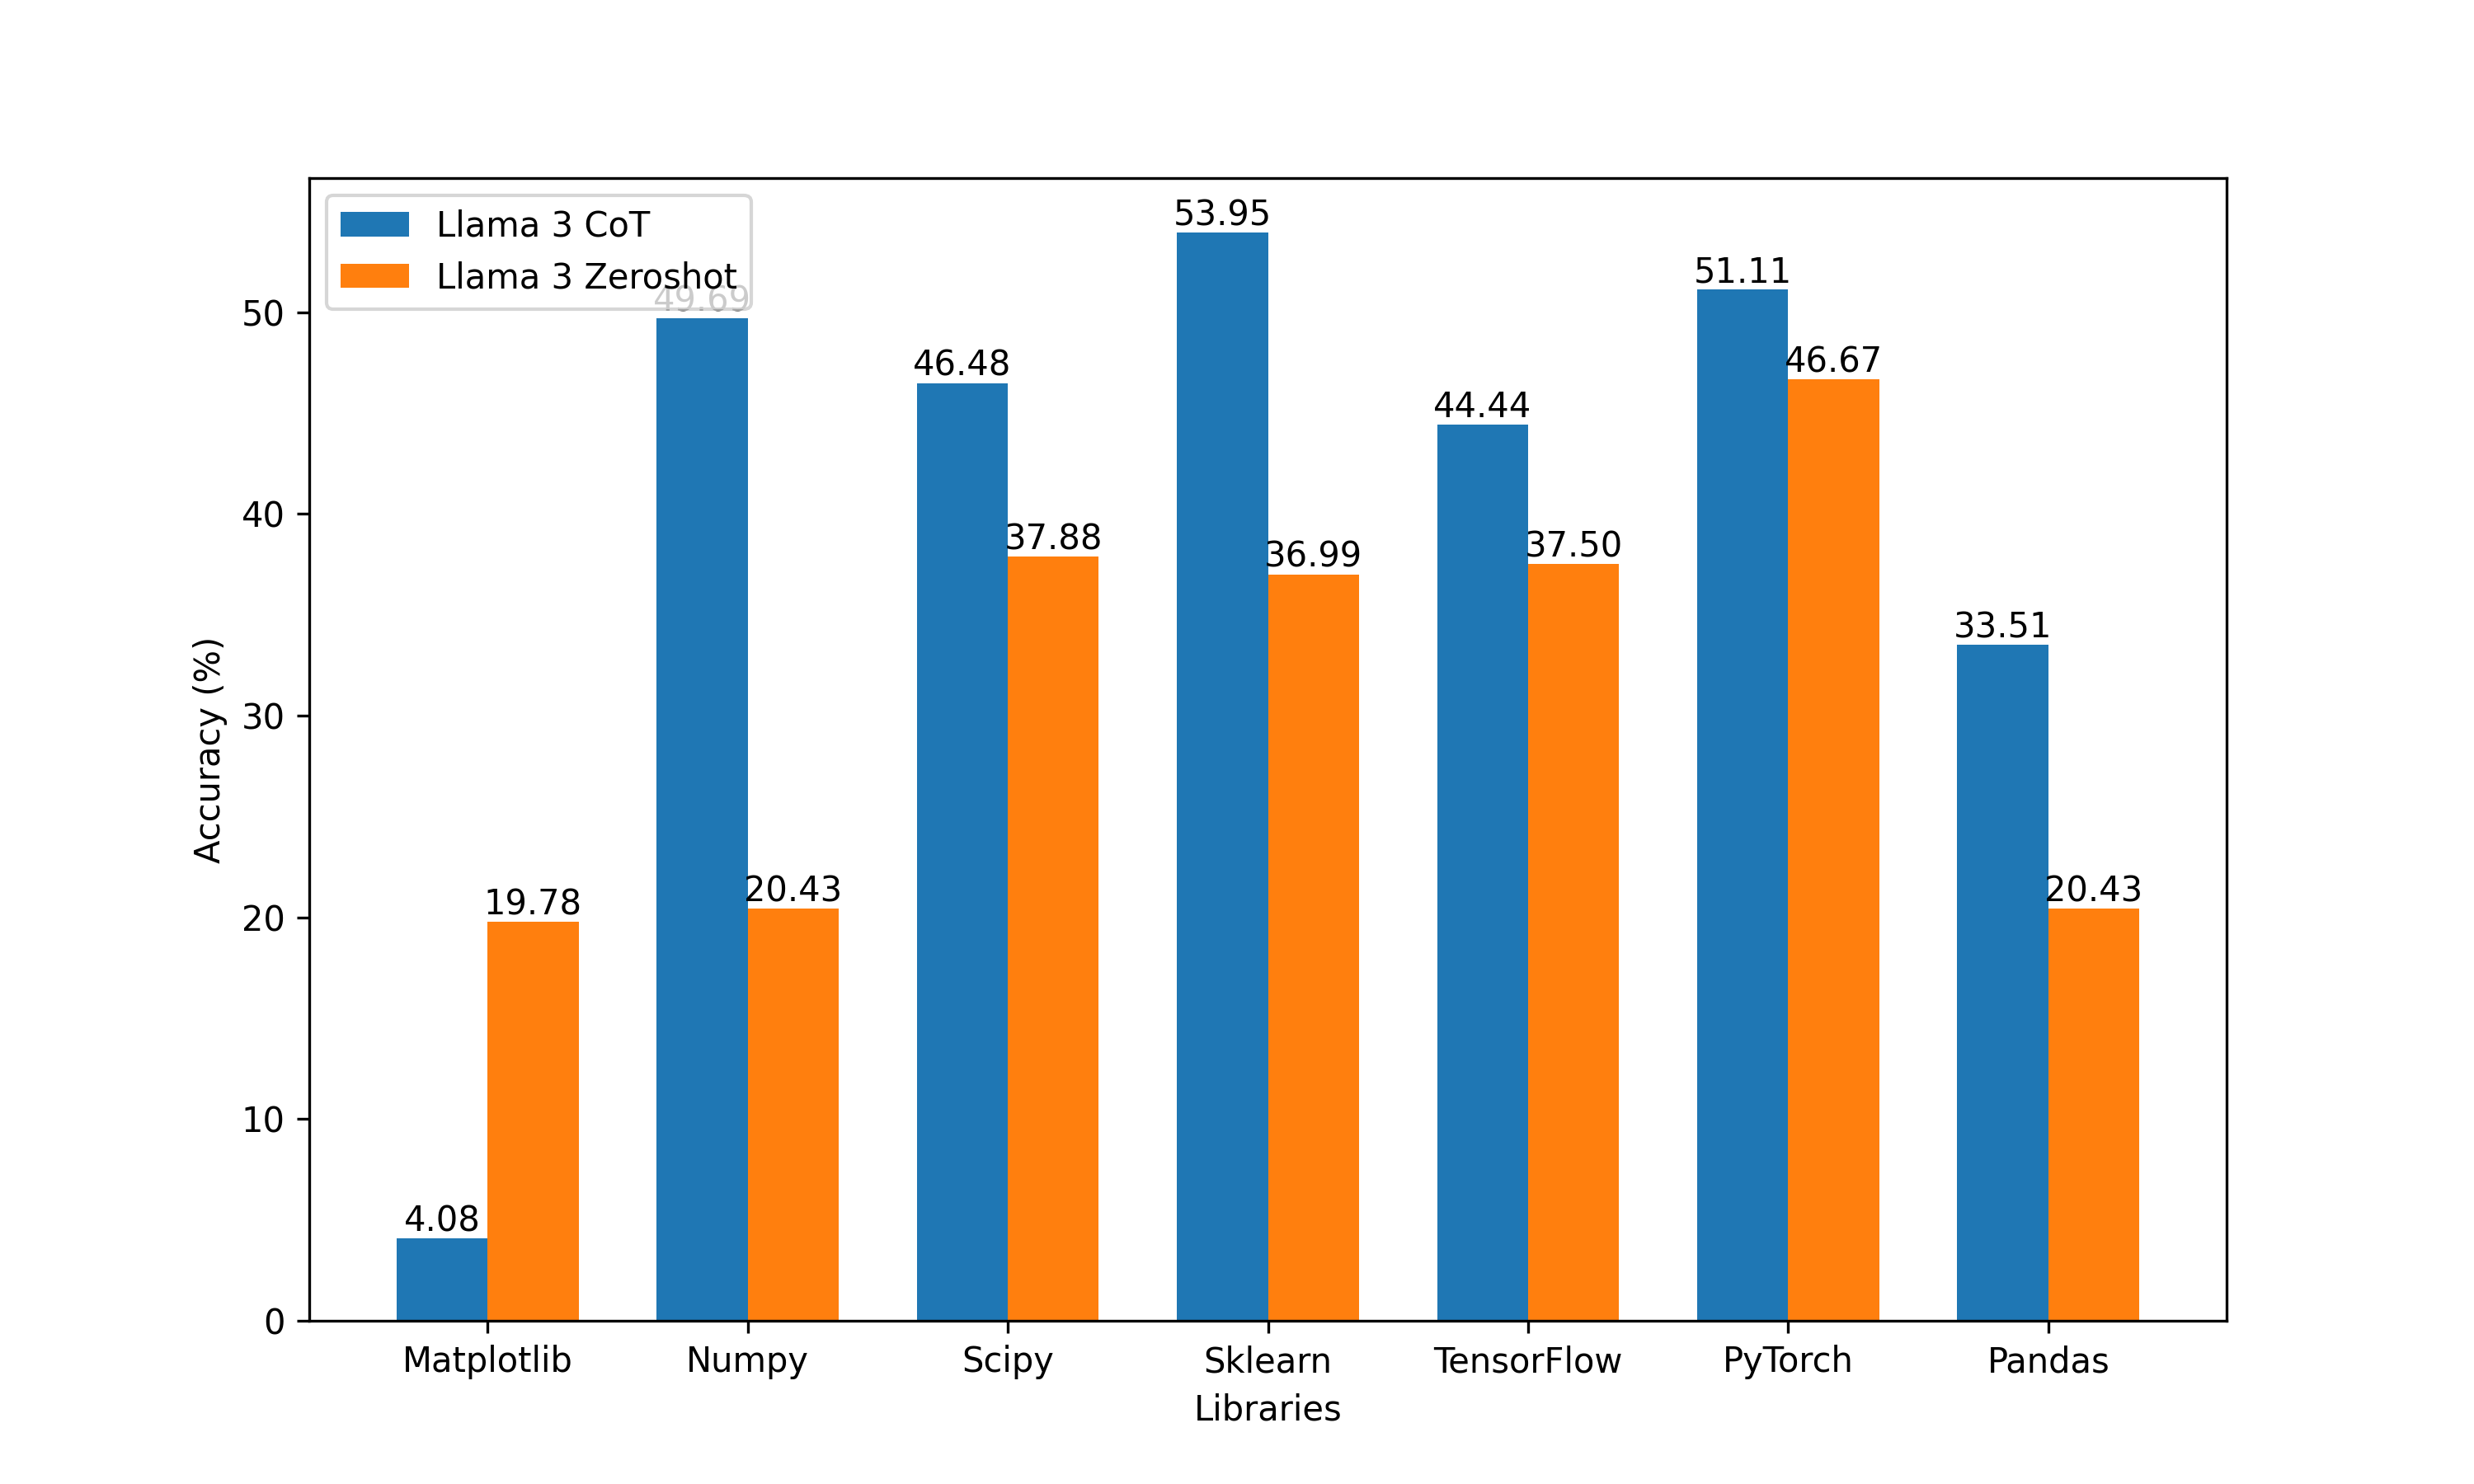
\includegraphics[width=\columnwidth]{img/code_llm}
        \caption*{Comparison of Llama 3 CoT and Zeroshot (without self-correction).}
    \end{figure}
\end{frame}

\section{Future Directions}

\begin{frame}{Performance vs. Number of Iterations}
    \textbf{Exploring Iterative Improvement:}
    \begin{itemize}
        \item In our current study, we conducted four types of experiments, each involving a single pass through 1000 problems due to cost constraints.

        \item Future research should investigate the relationship between performance and the number of maximum iterations.

        \item Understanding how performance scales with additional iterations could provide insights into the efficiency and effectiveness of iterative approaches.

        \item This could help in optimizing resource allocation for large-scale experiments and improving the overall performance of the CoT-SelfEvolve framework.
    \end{itemize}
\end{frame}

\begin{frame}{Using Metrics for Improvement}
    \begin{columns}
        \column{0.65\textwidth}
        \begin{itemize}
            \item \textbf{Current Limitation:} Each problem-solving attempt in CoT-SelfEvolve is treated as an independent instance.

            \item \textbf{Opportunity:} Leverage metadata (solution correctness, iterations, token cost) from these attempts.

            \item \textbf{Inspiration:} DSPy~\cite{khattab2023dspy} framework auto-optimizes prompts using:
                  \begin{enumerate}
                      \item Demonstrations based on labels and metrics.
                      \item Rewriting prompts and collecting metrics.
                  \end{enumerate}

            \item \textbf{Future Work:} Use collected metrics to select effective demonstrations for the Auto-CoT prompt generator.
        \end{itemize}

        \column{0.35\textwidth}
        \begin{figure}[H]
            \centering
            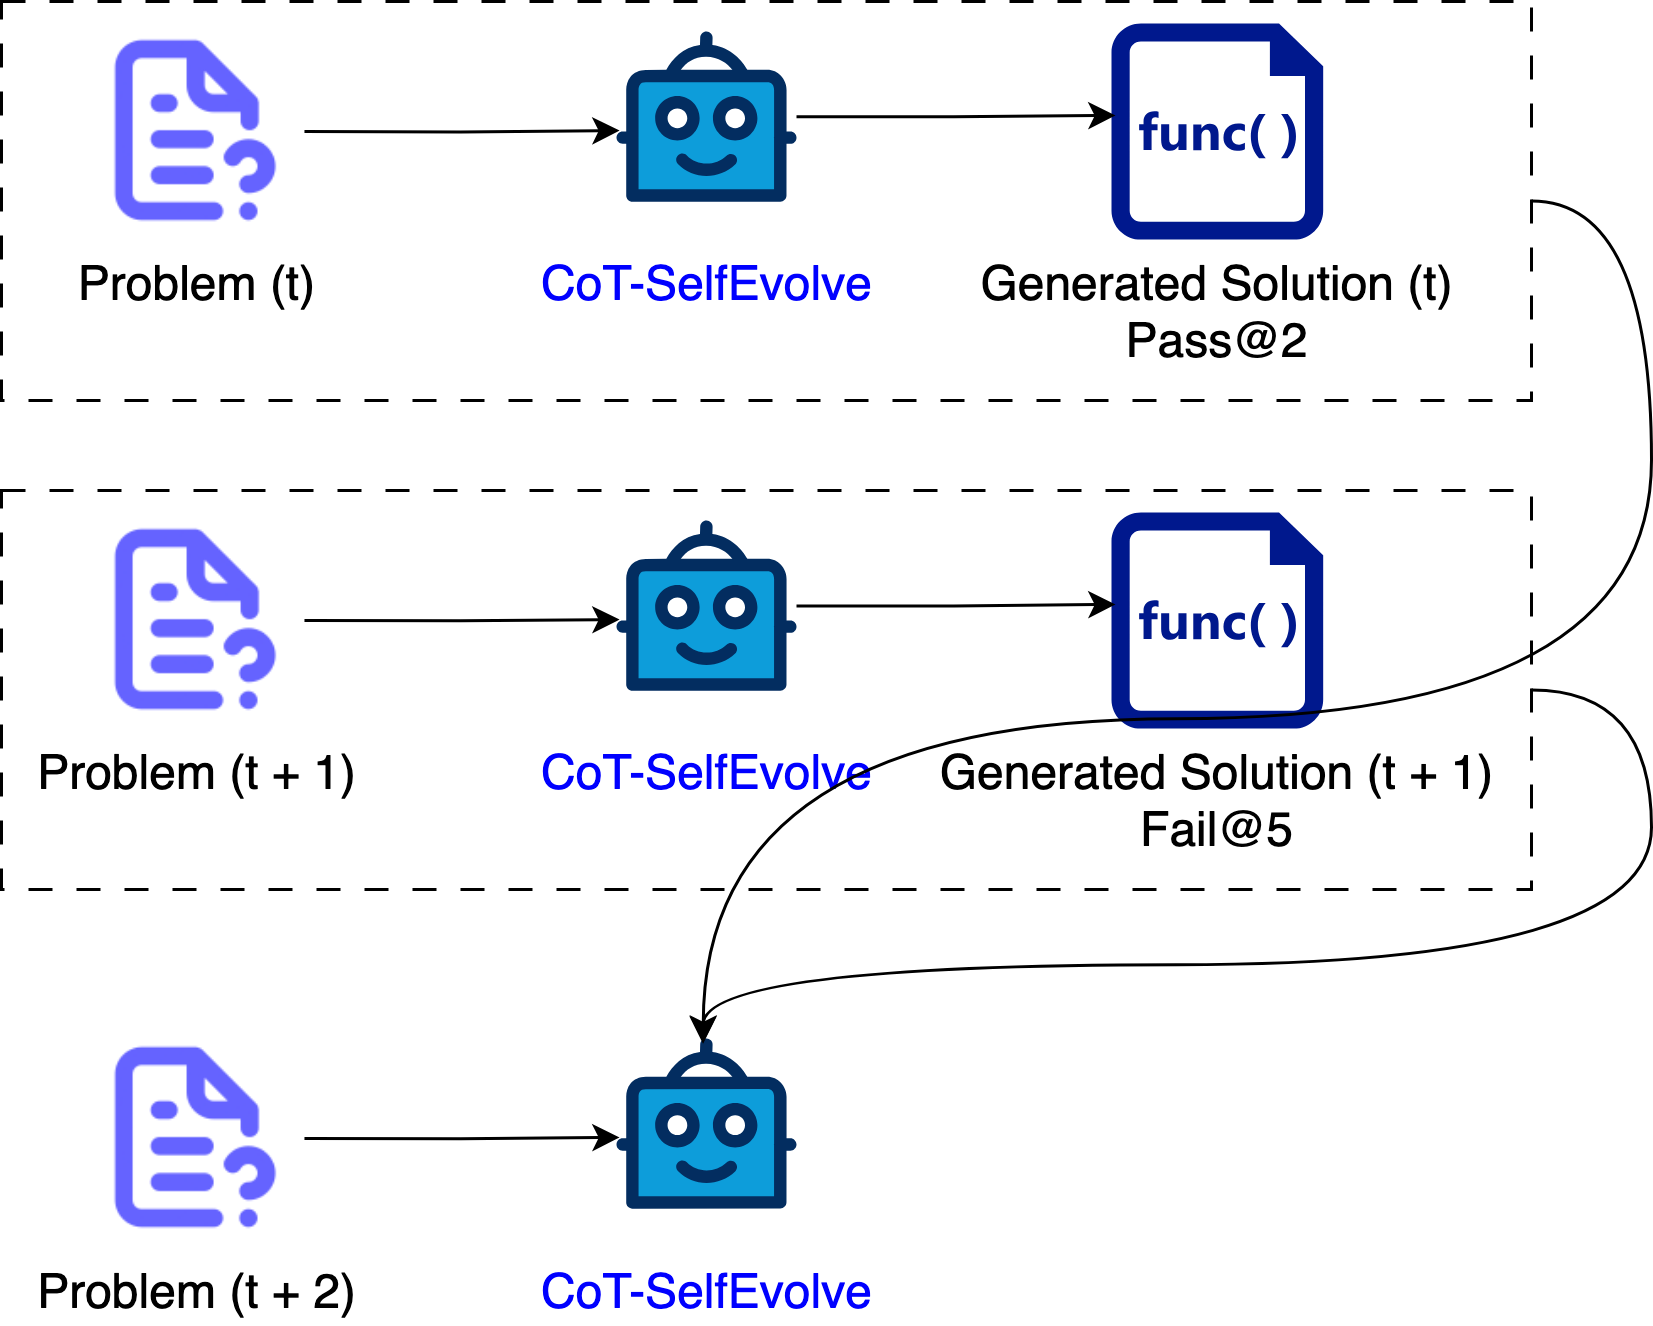
\includegraphics[width=\columnwidth]{img/enhanced_cot_selfevolve}
            \caption*{Leveraging metrics from prior runs to enhance CoT-SelfEvolve.}
        \end{figure}
    \end{columns}
\end{frame}

\section{Conclusion}

\begin{frame}{Conclusion}
    \begin{enumerate}
        \item The CoT-SelfEvolve model, leveraging LLMs like GPT-4, shows improved performance in handling Pytorch, Sklearn, and Matplotlib questions over the original SelfEvolve model.

        \item The ablation study verifies the significant role of CoT prompt generators in enhancing the model's performance, with a substantial relative gain of \textbf{16.39\%}.

        \item The potential of employing a larger LLM for guiding the code generation process is demonstrated, resulting in a significant performance increase, marked by a relative gain of \textbf{11.26\%}.
    \end{enumerate}
\end{frame}


\begin{frame}{Q\&A}
    \begin{figure}[!htb]
        \centering
        
\includegraphics[scale=1]{img/qna}
    \end{figure}
\end{frame}

\begin{frame}
    \begin{center}
        \Huge Thank you for your attention!
    \end{center}
\end{frame}

\section{Backup Slides}

\begin{frame}{Problems of LLMs}
    \begin{columns}[T]
        \begin{column}{0.70\textwidth}
            The works aimed at correcting LLMs can be classified according to the issues they tackle:
            \begin{enumerate}
                \item Hallucination: plausible-sounding but false information~\cite{gao2023rarr, zhang2023language}.

                \item Unfaithful Reasoning: derived conclusion does not follow the previously generated reasoning chain~\cite{he2022rethinking, pan2023logiclm}.

                \item Toxic Contents: content that is toxic, biased, or harmful due to biases present in the training datas~\cite{lu2022quark, gou2023critic}.

                \item Flawed Codes: flawed or incorrect code generation~\cite{chen2023teaching, olausson2023selfrepair}.
            \end{enumerate}
        \end{column}
        \begin{column}{0.30\textwidth}
            \begin{figure}[!htb]
                \centering
                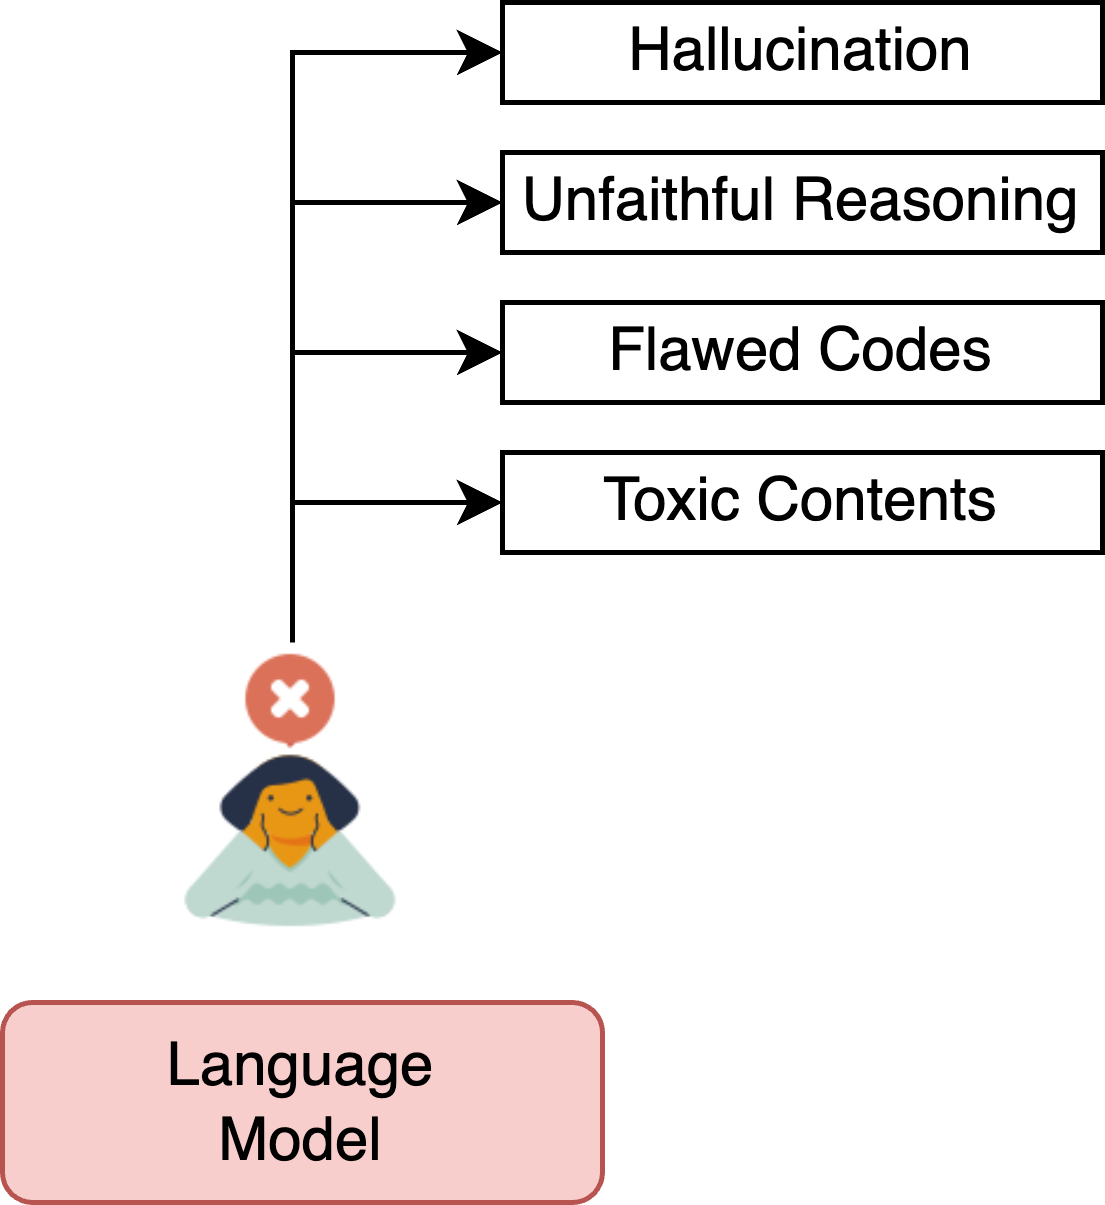
\includegraphics[width=1\textwidth]{img/language_model}
                \captionsetup{font=small,labelformat=empty}
                \caption{Problems of LLMs.}
            \end{figure}
        \end{column}
    \end{columns}
\end{frame}

\begin{frame}{Critic Model}
    \begin{columns}[T]
        \begin{column}{0.55\textwidth}
            Source of feedback:
            \begin{enumerate}
                \item Self-Feedback: the model itself generates feedback~\cite{weng2023large}.

                \item External Feedback: the model receives feedback from an external source (e.g., human, program executor and external knowledge)~\cite{gou2023critic}.
            \end{enumerate}

            Format of feedback:
            \begin{enumerate}
                \item Scalar Value: metrics based on pre-defined tests~\cite{weng2023large}.

                \item Natural Language: provides richer information than scalar value feedback~\cite{chen2023teaching}.
            \end{enumerate}
        \end{column}
        \begin{column}{0.45\textwidth}
            \begin{figure}[!htb]
                \centering
                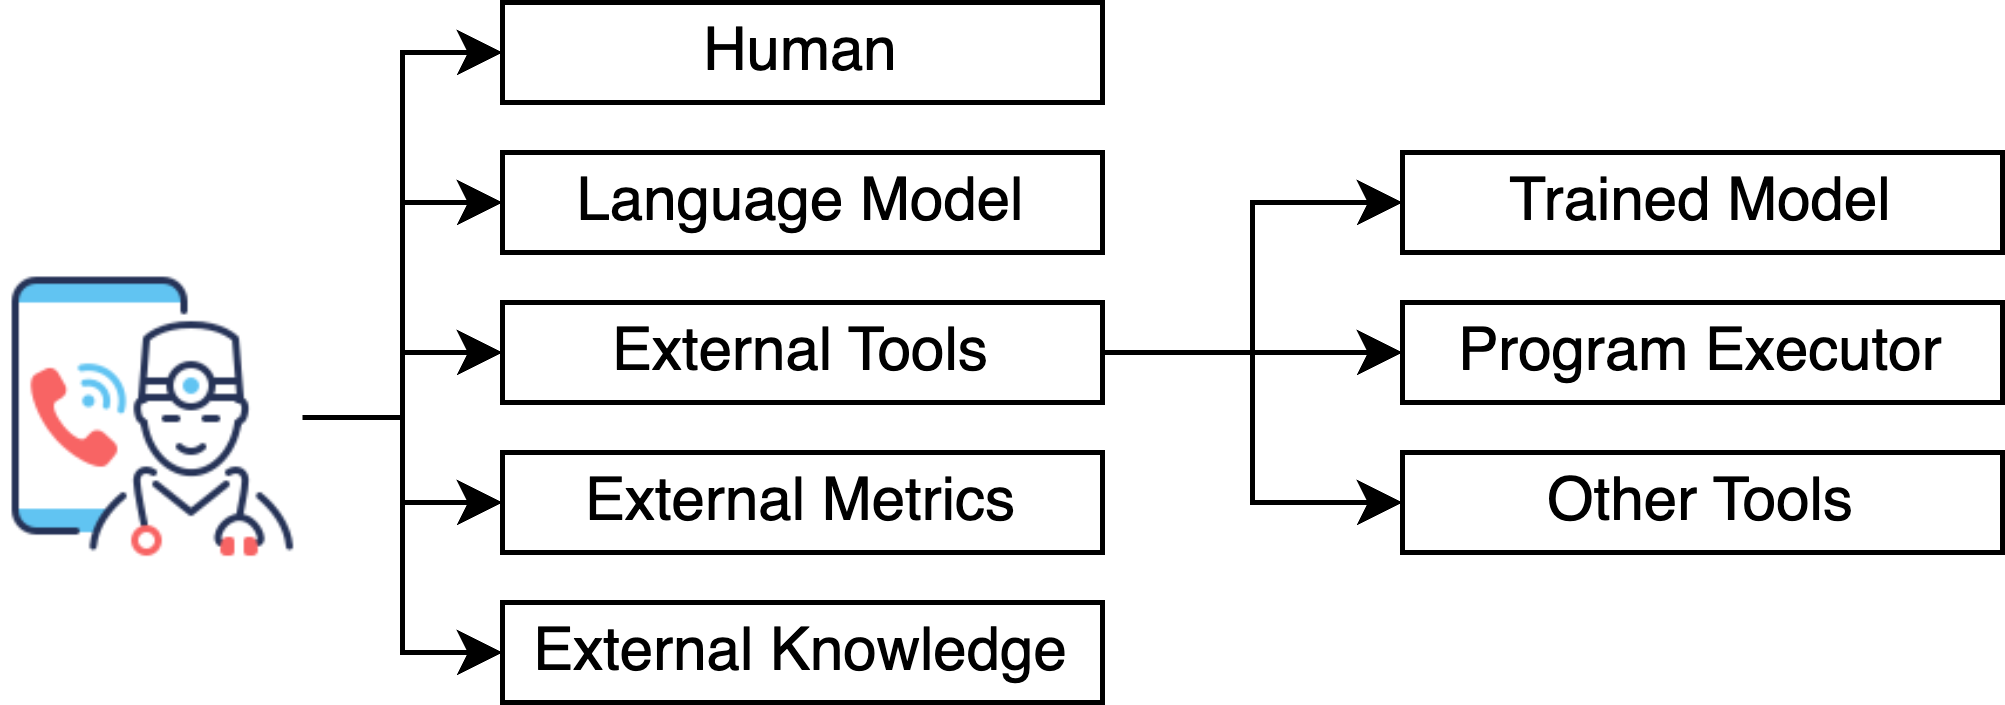
\includegraphics[width=1\textwidth]{img/critic_model}
                \captionsetup{font=small,labelformat=empty}
                \caption{Critic Model.}
            \end{figure}
        \end{column}
    \end{columns}
\end{frame}


\begin{frame}[allowframebreaks]{References}
    \bibliography{references}
\end{frame}

\end{document}
